\documentclass[12pt]{report}
\usepackage[spanish]{babel}
\usepackage[utf8]{inputenc}

\usepackage{graphicx,subcaption}
\usepackage{wrapfig, blindtext}
\usepackage{listings}
\usepackage{xcolor}
\usepackage{bookman}
\usepackage{underscore}
\usepackage[document]{ragged2e}
\setcounter{section}{+1}
\setcounter{figure}{-1}
% \ltset{
% 	backgroundcolor=\color{black!5},
% 	basicstyle=\footnotesize\ttfamily\small,
% }

\makeatletter
\renewcommand{\@makechapterhead}[1]{%
\vspace*{50 pt}%
{\setlength{\parindent}{0pt} \raggedright \normalfont
\bfseries\Huge
\ifnum \value{secnumdepth}>1 
    \if@mainmatter\thechapter.\ \fi%
\fi
#1\par\nobreak\vspace{40 pt}}}
\makeatother

\graphicspath{ {img/} }

\title{\textbf{Catharina van Hemessen}}
\author{Alberto Navalón Lillo, 3ESO A}

\begin{document}

\frontmatter
\maketitle
\tableofcontents
\mainmatter

\addcontentsline{toc}{chapter}{Introducción}

% Introduction chapter
\chapter*{Introducción}
\chaptermark{Introducción}

En este trabajo de investigación se van a tratar la vida y obras de la pintora flamenca renacentista Catharina van Hemessen (1528?-1587?), quien es reconocida como la primera pintora flamenca de la cual se conserva una obra extensa y, además, de autenticidad verificada. Principalmente se la conoce por series de pequeños retratos femeninos datados de entre finales de la década de 1540 y principios de la década de 1550.\bigskip


A van Hemessen se la distingue por haber creado el primer autorretrato femenino conocido, su \textit{Autorretrato} (figura 0), datado en 1548, además por la propia autora, que escribió las siguientes palabras sobre el lienzo:\bigskip

\indent``\textit{Yo, Catharina van Hemessen, me he retratado a mí misma} / \textit{1548} / \textit{Ella de 20 años de edad}''\footnote{Del original: ``\textit{Ego Catarina de / Hemessen me / pinxi \textbf{1548} // Etatis suae / 20}''}\bigskip

Este retrato muestra a la artista en las fases tempranas de la creación de un retrato. En la actualidad, la obra pertenece a la colección del Kunstmuseum Basel, al que pertenece la mayor y más significativa colección pública de arte en Suiza. También podemos encontrar obras de van Hemessen en el Rijksmuseum de Ámsterdam y en la National Gallery de Londres.\bigskip

Como Catharina, muchas otras mujeres de su tiempo soñaban con ser pintoras y artistas. Sin embargo, no era un sueño fácil de conseguir para ellas, dado que su educación artística implicaría, entre otras cosas, la disección de cadáveres humanos y el estudio de la figura del cuerpo del hombre, lo que constituía una educación poco accesible a las mujeres, además de no muy placentera. Todo esto en adición a la discriminación hacia ellas, quienes eran consideradas incapaces de trabajar como artistas.\bigskip

\begin{wrapfigure}{l}{0.4\textwidth}
	\begin{center}
		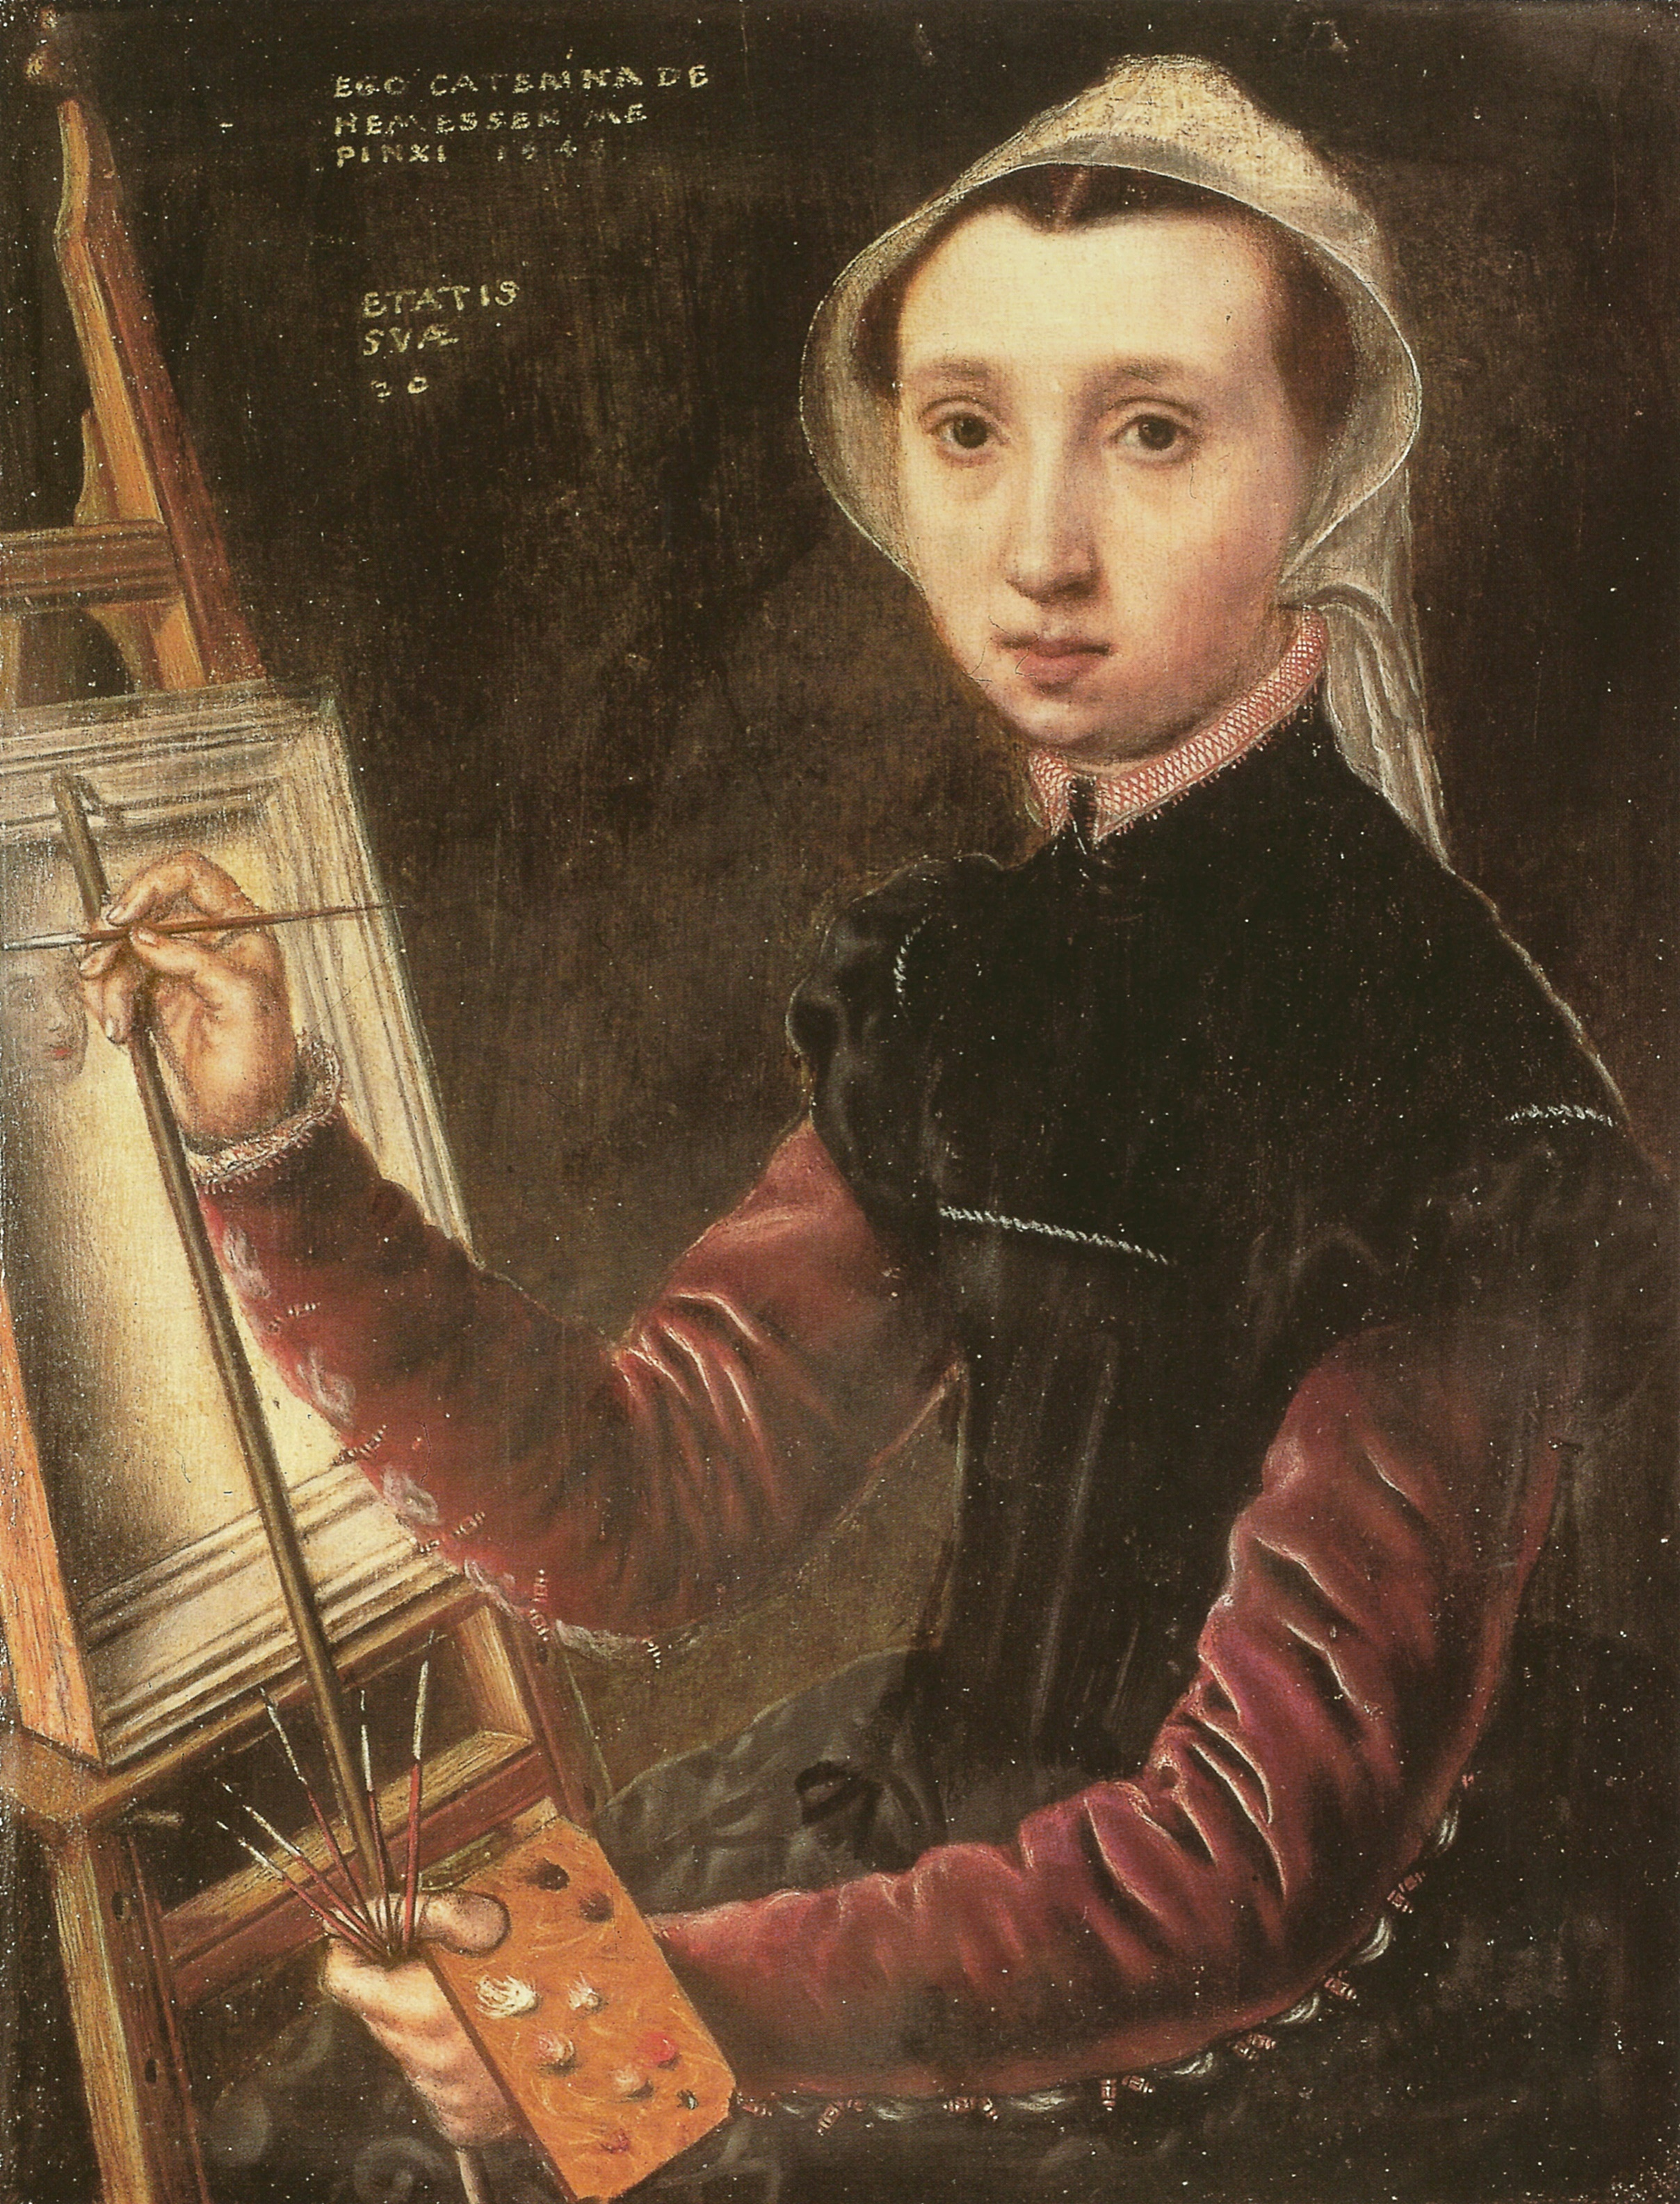
\includegraphics[width=0.9\linewidth]{self-portrait}
		\caption{\textit{Autorretrato}, Catharina van Hemessen, 1548}
		\label{fig:wrapfig}
	\end{center}
\end{wrapfigure}

En adición a esto, el período de aprendizaje de los artistas en esta época también consistía en vivir durante cuatro o cinco años junto a un artista más veterano, quien le pudiese enseñar de primera mano. Por ello, pocas llegaban a esto, puesto que muy pocos artistas veteranos aceptarían en aquel entonces a una mujer como aprendiz; y las que realmente conseguían recibir esta educación, como es el caso de van Hemessen, lo hacían de parte de alguien cercano a ellos. Catharina fue instruida por su propio padre, Jan Sanders van Hemessen, un reputado pintor.\bigskip

Actualmente se ha identificado un total de 10 obras firmadas y datadas por la propia artista, entre las que se encuentran seis retratos, un autorretrato (su \textit{Autorretrato}), y pinturas religiosas en las que se muestran grandes grupos de figuras. Un ejemplo de su obra religiosa es su \textit{Cristo se encuentra a Verónica} (1541-1560), en que se representa la imagen bíblica de la Santa Faz.

% Biography
\chapter{Biografía}

Catharina van Hemessen nació en Amberes (Bélgica), muy probablemente en el año 1528, hija de Bárbara de Fevre, quien a su vez fue hija de un rico comerciante de la ciudad; y del pintor manierista y alumno del gran pintor y grabador flamenco Hendrick van Cleve, Jan Sanders Van Hemessen (Hemiksen, 1500?-Haarlem, 1566?). De este fue, presumiblemente, además de hija, aprendiz y discípula, y supuestamente colaboró con él en muchas de sus obras, como era costumbre en muchas mujeres artistas de la época. Formó parte del círculo de la corte hacia 1540, cuando entró junto a su padre, bajo el patronazgo de la reina María de Hungría (figura 1.1), de quien fue dama de honor.\bigskip

\begin{wrapfigure}{r}{0.4\textwidth}
	\begin{center}
		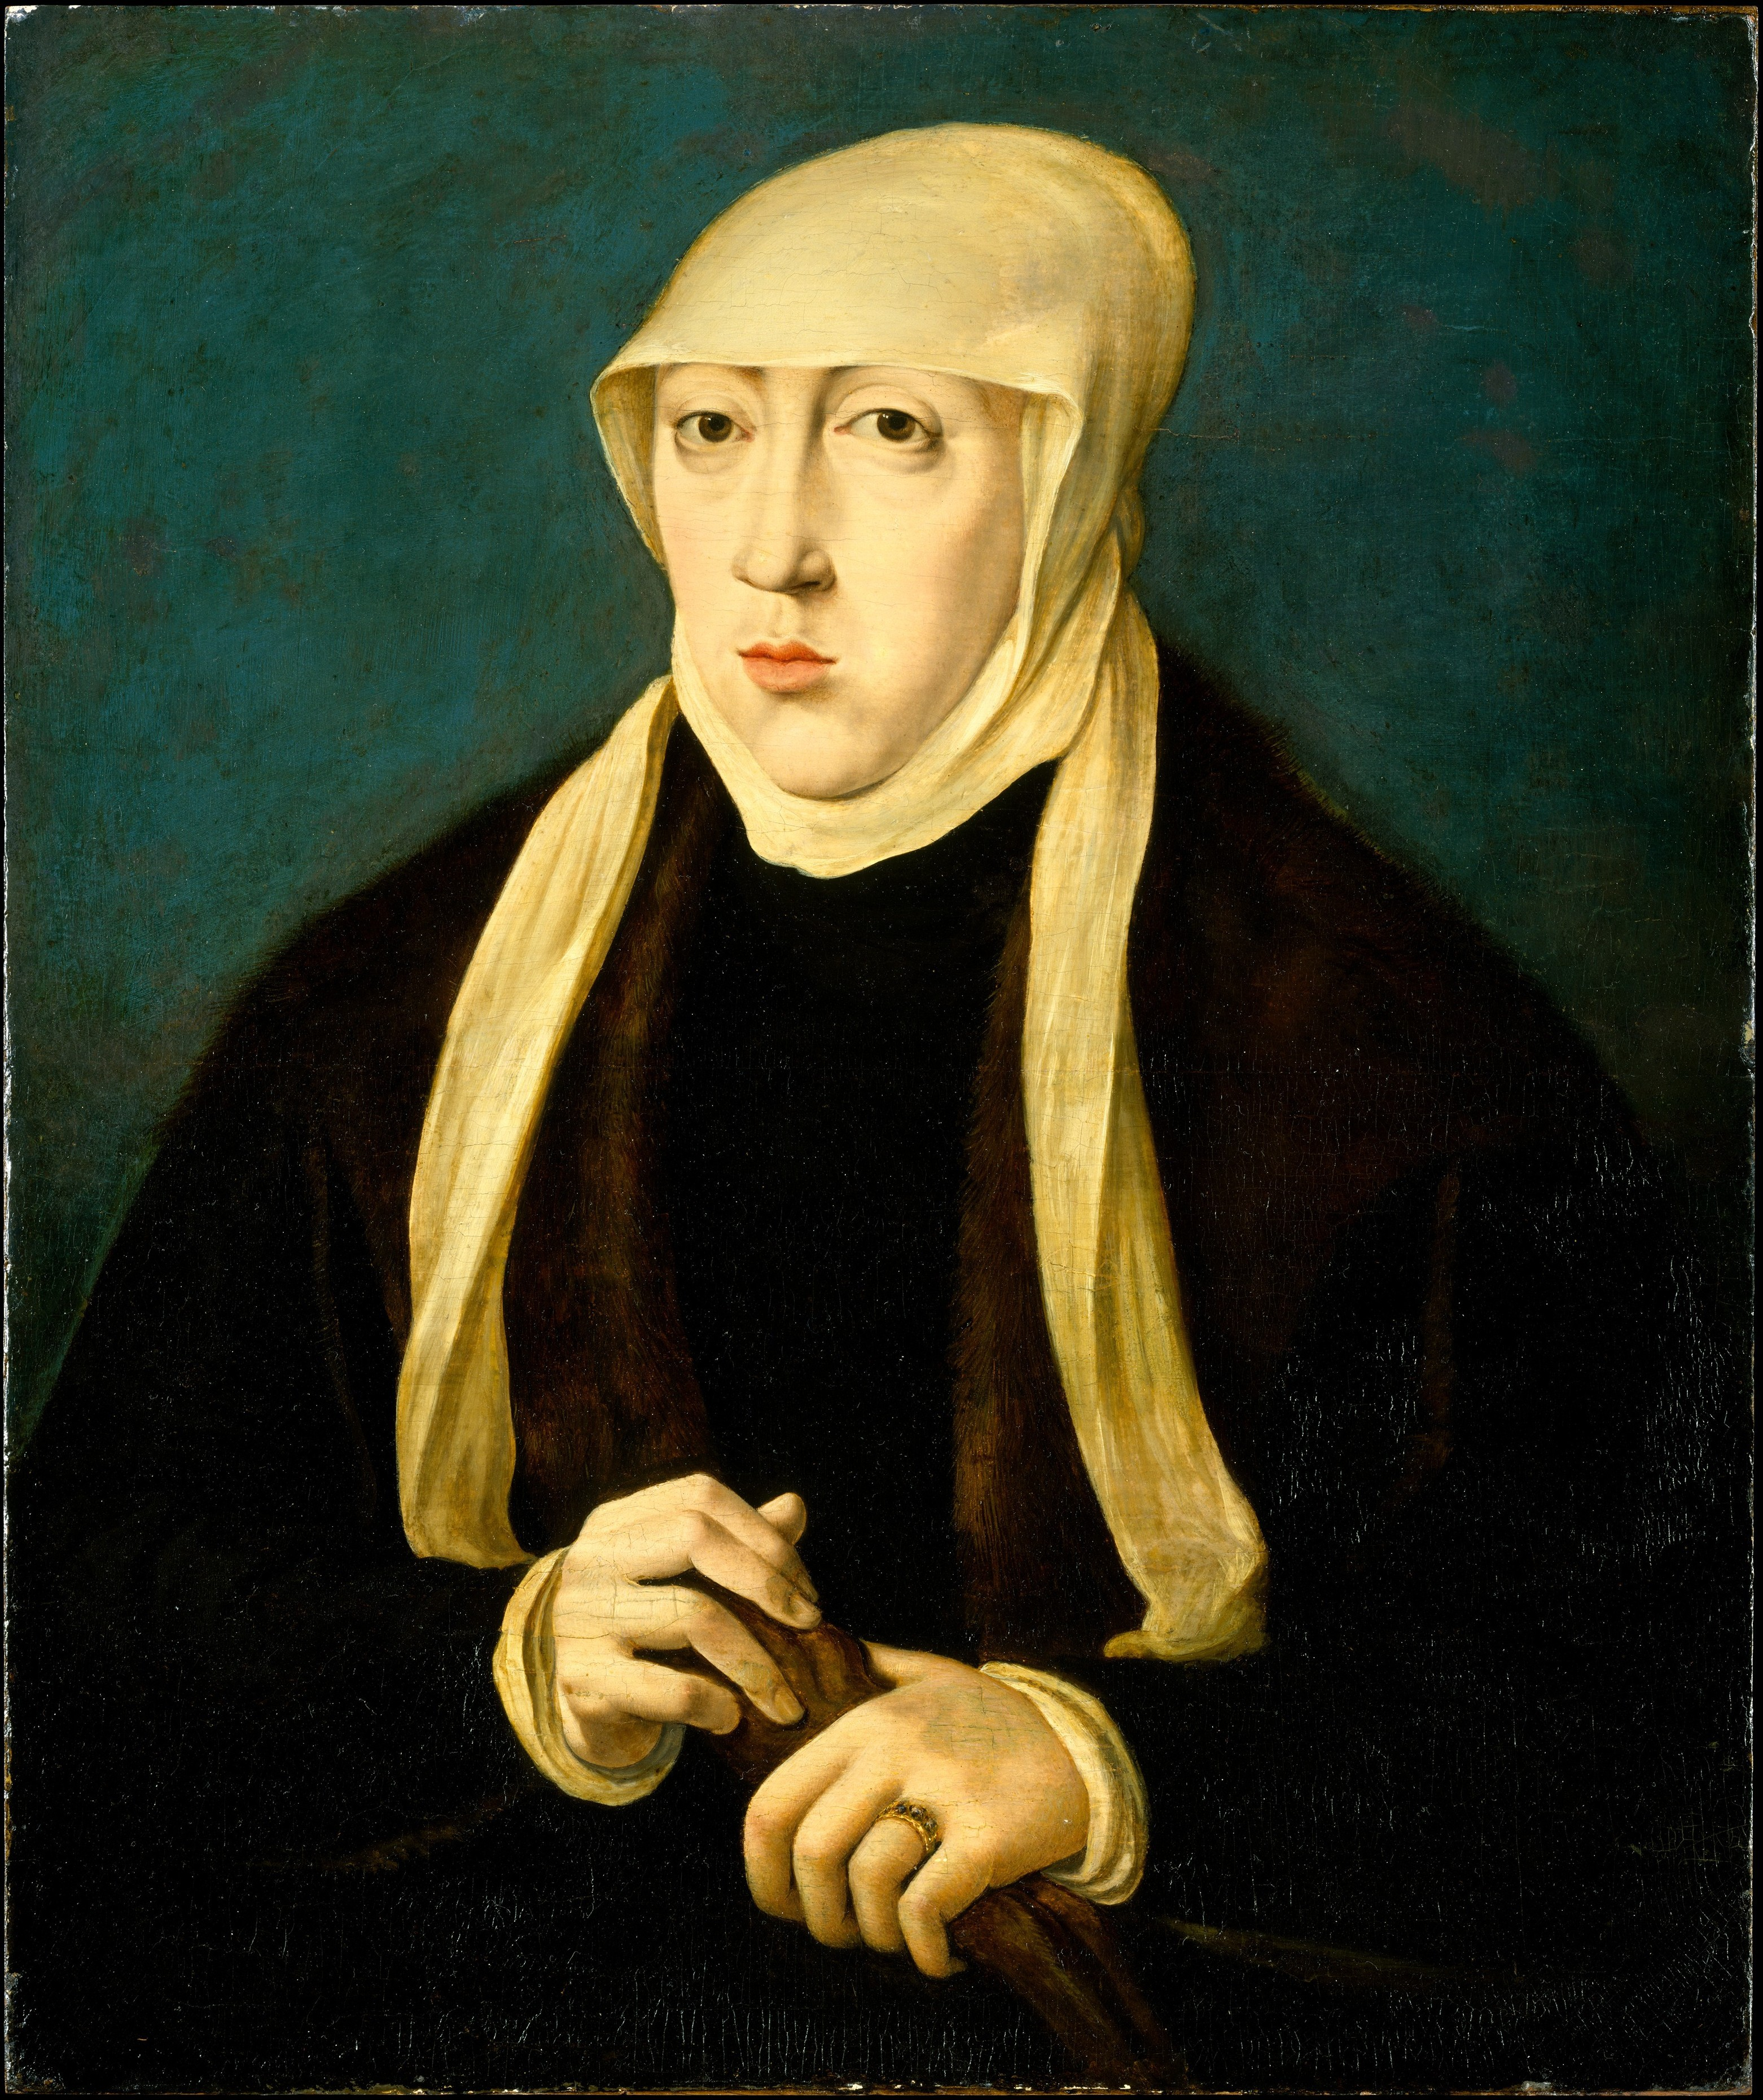
\includegraphics[width=0.9\linewidth]{mary-queen-of-hungary}
		\caption{María de Hungría, Habsburgo y Austria (1505-1558)}
		\label{fig:wrapfig}
	\end{center}
\end{wrapfigure}

En 1554, con aproximadamente 26 años, contrae matrimonio con Chrétien de Morien, el organista de la catedral de Amberes, cargo considerado importante en aquella época. A consecuencia de esto, su carrera artística se frena, seguramente para dedicarse exclusivamente a su matrimonio, dado que no se han hallado trabajos suyos datados a partir de esa época, con una única excepción de la que se tiene constancia, que será explicada a continuación.\bigskip

Sin embargo, cuando poco tiempo después María de Hungría renunció a la regencia y se marchó a vivir a España, Catharina y su marido se marcharon con ella, y disfrutaron de una vida más o menos acomodada gracias a la ayuda económica de la hermana del emperador.\bigskip

En el poco tiempo que la pareja quedó en España, es sabido que van Hemessen volvió a coger el pincel para colaborar en la creación del retablo de Tendilla del Monasterio Jerónimo de Santa Ana de Guadalajara. Tras analizar las pinturas del retablo se dedujo que fueron obra de cuatro pintores, además de Catharina, del taller de Jan Sanders van Hemessen. En 1915, tras su reaparición, fue adquirido por el Cincinnati Art Museum (EEUU).\bigskip

\begin{figure}[h]
	\centering
	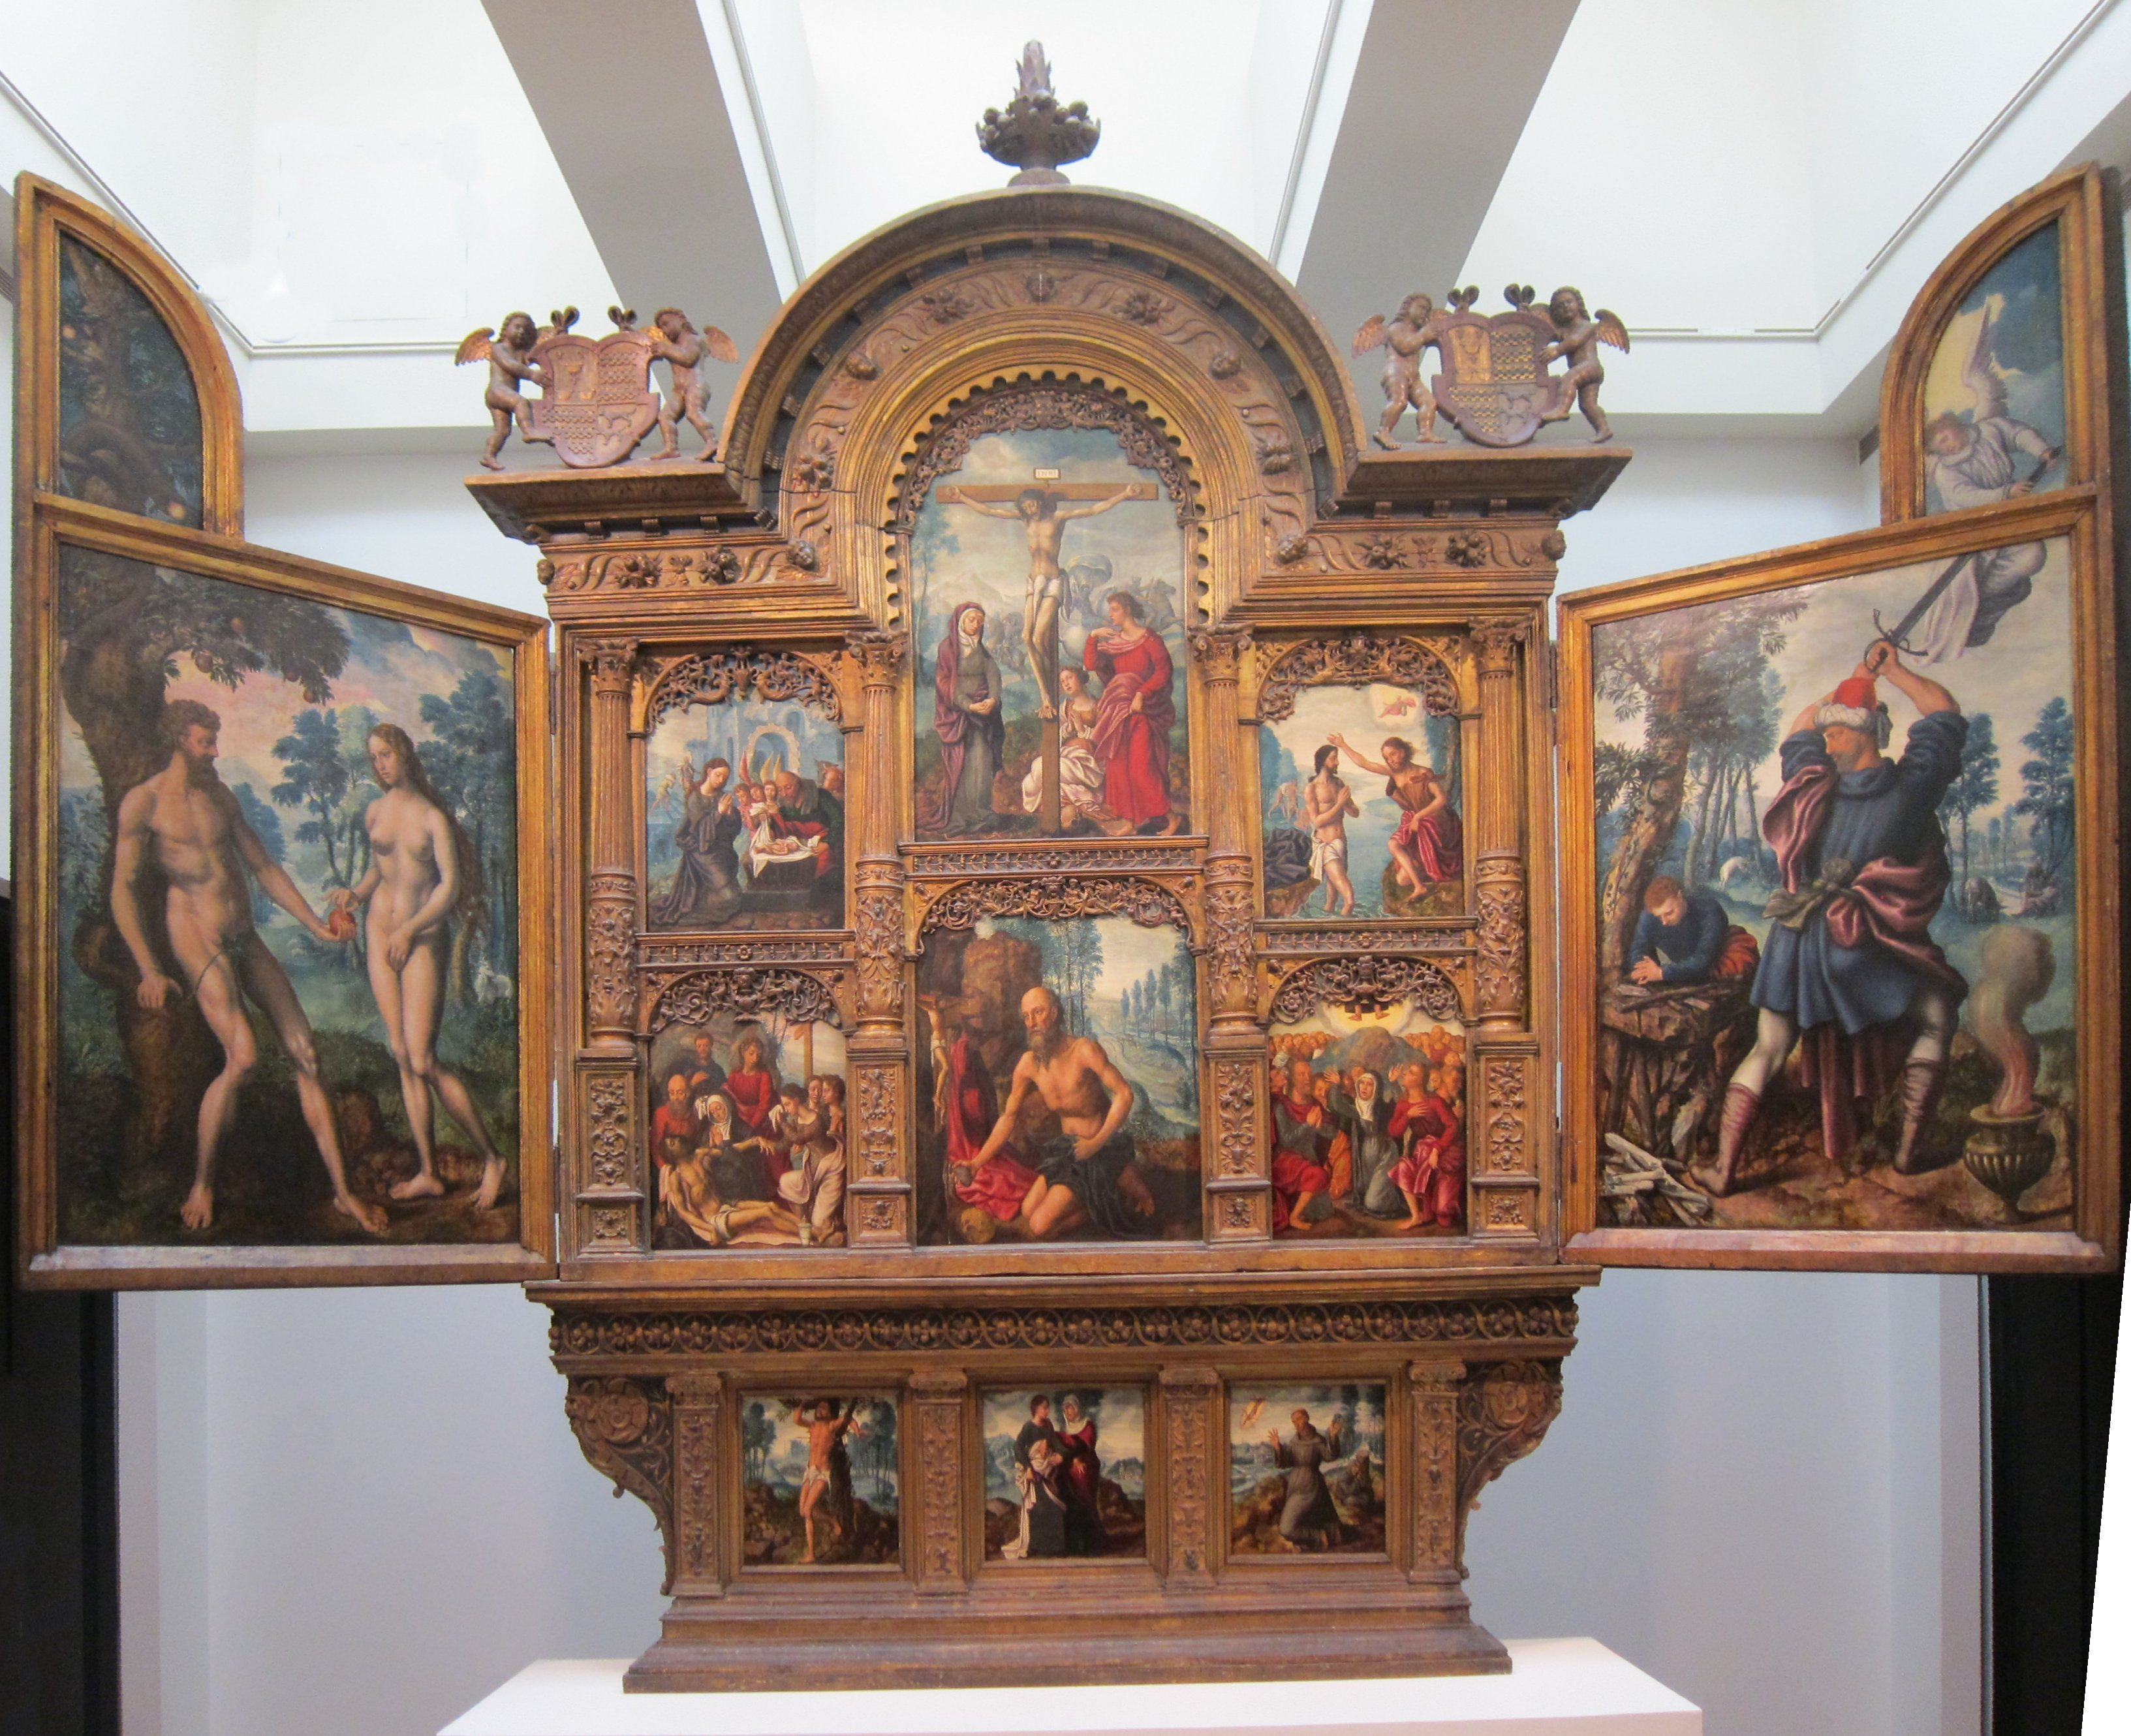
\includegraphics[width=0.75\linewidth]{retablo-de-tendilla}
	\caption{Retablo de Tendilla, Cincinnati Art Museum}
	\label{fig:wrapfig}
\end{figure}

Hacia finales del año 1558, tras la muerte de su protectora, la reina María de Hungría, la pareja volvió a Países Bajos, y se establecieron en su ciudad natal, Amberes. Ya en 1565, aún estando la pareja sin ningún hijo, Chrétien recibió una oferta para trabajar en 's-Hertogenbosch, por lo que decidieron mudarse allí. A partir de entonces, nada más se sabe de su vida, aparte de que (aunque no es completamente seguro) Catharina van Hemessen falleció por causas naturales en el año 1587, a los 60 años de edad.

\section{Reconocimiento}

A lo largo de su vida, van Hemessen fue mencionada en las respectivas obras de dos biógrafos italianos de artistas:
\begin{itemize}
	\item En la \textit{Descripción de los Países Bajos}\footnote{Del original, en italiano: \textit{Descrittione di Tutti i Paesi Bassi}}, de Lodovico Guicciardini, 1567.
	\item En las \textit{Vidas}\footnote{Del orig., en italiano: \textit{Le vite de' più eccellenti pittori, scultori, e architettori}}, de Giorgio Vasari, 1568.
\end{itemize}

Estas dos menciones implican que, en vida, Catharina van Hemessen gozó de éxito y una popularidad notorios dentro del mundo artístico, y es por ello que la reina María de Hungría confió en ella para formar parte de la corte y ser retratista allí. Esto se debe en gran parte a que su padre fue un artista de gran renombre, lo que es en parte negativo, dado que las pocas mujeres que llegaban a gozar de este reconocimiento no lo hacían por mérito propio, sino que eran otras personas cercanas ya conocidas las que influían en los pensamientos hacia dicha mujer, completamente ajenos a su capacidad artística real.

\section{Trabajo como pintora y retratista}

A pesar de que van Hemessen creó al menos dos obras de carácter religioso, ella era principalmente una retratista, creando la gran mayoría de sus obras como tal. Ocho retratos pequeños y dos pinturas de carácter religioso, todos datados entre 1548 y 1552, y con su firma inscrita han sobrevivido hasta nuestros días. Catharina retrató ostensiblemente a personas nobles y adineradas, tanto hombres como mujeres, normalmente frente a un fondo oscuro. Las figuras delicadas que pintaba eran de apariencia elegante y provistas de trajes y accesorios estilosos.\bigskip

Su obra más conocida es su \textit{Autorretrato}, mencionado anteriormente. Alrededor del mismo tiempo en que su \textit{Autorretrato} fue firmado (1548), Catharina van Hemessen pintó otra de sus obras más famosas: \textit{Retrato de una mujer de 22 años tocando la espineta} (1548), el cual podría ser un retrato de su hermana.\bigskip

Los retratos de van Hemessen se caracterizan por su realismo. Tanto su autorretrato como la media docena de retratos restante atribuidos a ella son obras pequeñas y calmadas. Los retratados, usualmente sentados, se representan frente a un fondo oscuro o neutro, y sus miradas rara vez se encuentran con los ojos del espectador.\bigskip

\chapter{Trabajos notables}

En este apartado se van a mostrar algunas de las obras más relevantes de Catharina van Hemessen, junto con alguna información cuando sea posible aportarla. Todas ellas están ordenadas en orden cronológico.

\section{\textit{Autorretrato}}

\textsc{Figura 3.1} (Galería de obras).\bigskip

Esta es posiblemente la obra más famosa de la artista flamenca. En ella se representa a la propia Catharina al comienzo de la creación de uno de sus retratos.
\begin{itemize}
	\item \textbf{Fecha}: 1548
	\item \textbf{Dimensiones}: 33x26,5 cm
	\item \textbf{Técnica}: pintura al óleo
	\item \textbf{Colección}: Kunstmuseum Basel, Basilea, Suiza
\end{itemize}

\section{\textit{Retrato de una mujer de 22 años tocando la espineta}}

\textsc{Figura 3.2} (Galería de obras).\bigskip

Se trata de una de sus obras más populares. Se dice que la mujer representada tocando la espineta (un instrumento precursor del piano, típico del período renacentista) es la hermana de Catharina, que fue música.
\begin{itemize}
	\item \textbf{Fecha}: 1548
	\item \textbf{Dimensiones}: 30,5x24 cm
	\item \textbf{Técnica}: pintura al óleo
	\item \textbf{Colección}: Wallraf-Richartz-Museum, Colonia, Alemania
\end{itemize}

\section{\textit{Retrato de una mujer, probablemente un autorretrato}}

\textsc{Figura 3.3} (Galería de obras).\bigskip

Esta obra es considerada en parte como un autorretrato de van Hemessen, aunque los rasgos de la persona representada difieren notablemente respecto a los de ella misma en su \textit{Autorretrato}. Por ello, no se puede verificar este hecho.
\begin{itemize}
	\item \textbf{Fecha}: 1548
	\item \textbf{Dimensiones}: 23x15,2 cm
	\item \textbf{Técnica}: pintura al óleo sobre tabla
	\item \textbf{Colección}: Rijksmuseum, Ámsterdam, Países Bajos
\end{itemize}

\section{\textit{Retrato de una mujer de 30 años}}

\textsc{Figura 3.4} (Galería de obras).\bigskip

Se dice que esta obra está emparejada con el \textit{Retrato de un hombre de 42 años}, dada su gran similitud, mismo tamaño y misma fecha de creación.
\begin{itemize}
	\item \textbf{Fecha}: 1549
	\item \textbf{Dimensiones}: 22x17 cm
	\item \textbf{Técnica}: pintura al óleo
	\item \textbf{Colección}: Musées Royaux des Beaux-Arts de Belgique, Bruselas, Bélgica
\end{itemize}

\section{\textit{Retrato de un hombre de 42 años}}

\textsc{Figura 3.5} (Galería de obras).\bigskip

Pareja de la obra anterior.
\begin{itemize}
	\item \textbf{Fecha}: 1549
	\item \textbf{Dimensiones}: 22x17 cm
	\item \textbf{Técnica}: pintura al óleo
	\item \textbf{Colección}: Musées Royaux des Beaux-Arts de Belgique, Bruselas, Bélgica
\end{itemize}

\section{\textit{Retrato de una joven dama}}

\textsc{Figura 3.6} (Galería de obras).\bigskip

\begin{itemize}
	\item \textbf{Fecha}: 1551
	\item \textbf{Dimensiones}: 40,9x30,1 cm
	\item \textbf{Técnica}: pintura al óleo
	\item \textbf{Colección}: Bowes Museum, Barnard Castle, Reino Unido
\end{itemize}

\section{\textit{Retrato de una mujer con un perro}}

\textsc{Figura 3.7} (Galería de obras).\bigskip

La retratada, que lleva un perro consigo bajo el brazo, no ha sido identificada, aunque se puede observar con claridad que se trataba de una mujer adinerada, puesto que la vestimenta refleja este hecho.
\begin{itemize}
	\item \textbf{Fecha}: 1551
	\item \textbf{Dimensiones}: 22,9x17,8 cm
	\item \textbf{Técnica}: pintura al óleo sobre tabla de roble
	\item \textbf{Colección}: National Gallery, Londres, Reino Unido
\end{itemize}

\section{Predela del retablo de Tendilla}

\textsc{Figura 3.8} (Galería de obras).\bigskip

Este es un retablo con escenas del Antiguo y del Nuevo Testamento. Aunque se dice que participaron al menos cuatro personas en su creación, solo se citan a dos: a Catharina y a su padre.
\begin{itemize}
	\item \textbf{Fecha}: principios de la década de 1550
	\item \textbf{Dimensiones}: 355x457,2 cm (retablo)
	\item \textbf{Técnica}: pintura al óleo sobre tabla
	\item \textbf{Colección}: Cincinnati Art Museum, Cincinnati, OH, EEUU
\end{itemize}

\section{\textit{Retrato de una mujer}}

\textsc{Figura 3.9} (Galería de obras).\bigskip

\begin{itemize}
	\item \textbf{Fecha}: ¿principios de la década de 1550? / ¿1555?
	\item \textbf{Dimensiones}: 33x25 cm
	\item \textbf{Técnica}: pintura al óleo
	\item \textbf{Colección}: Fitzwilliam Museum, Londres, Reino Unido
\end{itemize}

\section{\textit{Retrato de un hombre}}

\textsc{Figura 3.10} (Galería de obras).\bigskip

Al igual que el \textit{Retrato de una mujer con un perro} (por eso se clasifican de la misma forma), no se conoce la identidad del retratado, aunque se puede determinar que se trataba de una hombre adinerado, tal y como lo muestran, entre otros, su vestimenta y su espada dorada.
\begin{itemize}
	\item \textbf{Fecha}: 1552
	\item \textbf{Dimensiones}: 36,2x29,2 cm
	\item \textbf{Técnica}: pintura al óleo sobre tabla de roble
	\item \textbf{Colección}: National Gallery, Londres, Reino Unido
\end{itemize}

\section{\textit{Retrato de un niño}}

\textsc{Figura 3.11} (Galería de obras).\bigskip

Esta obra no tiene un autor confirmado, pero se atribuye mayoritariamente a Catharina van Hemessen, principalmente por el estilo utilizado, y la naturaleza de las figuras. También podemos observar la presencia de un pequeño pájaro que se posa sobre la mano de un niño.
\begin{itemize}
	\item \textbf{Fecha}: 1559
	\item \textbf{Dimensiones}: 19,7x14,6 cm
	\item \textbf{Técnica}: pintura al óleo sobre tabla
	\item \textbf{Colección}: colección privada
\end{itemize}

\section{\textit{Retrato de una joven dama}}

\textsc{Figura 3.12} (Galería de obras).\bigskip

\begin{itemize}
	\item \textbf{Fecha}: 1560
	\item \textbf{Dimensiones}: 30,5x22,9 cm
	\item \textbf{Técnica}: desconocida
	\item \textbf{Colección}: Baltimore Museum of Art, Baltimore, MD, EEUU
\end{itemize}

\section{\textit{Cristo se encuentra a Verónica}}

\textsc{Figura 3.13} (Galería de obras).\bigskip

Esta es probablemente la obra religiosa más conocida de Catharina van Hemessen. Destaca el cambio de estilo: de un estilo sencillo y relajado a una escena tan cargada como es la que en esta obra se representa.
\begin{itemize}
	\item \textbf{Fecha}: ¿1541?-¿1560?
	\item \textbf{Dimensiones}: 38x28 cm
	\item \textbf{Técnica}: pintura al óleo sobre panel
	\item \textbf{Colección}: colección privada
\end{itemize}

\chapter{Galería de obras}

Aquí se presentan en forma de imagen las trece obras mencionadas anteriormente. Todas ellas están ordenadas de la misma forma que en el apartado anterior, esto es, en orden cronológico.\bigskip

\underline{\textbf{Aviso de copyright}}: TODAS LAS IMÁGENES, TANTO ESTAS COMO LAS USADAS ANTERIORMENTE, SON O BIEN DE DOMINIO PÚBLICO, O BIEN SU LICENCIA DE CREATIVE COMMONS PERMITE EL USO DE LAS MISMAS, YA QUE SE HAN DEDICADO AL DOMINIO PÚBLICO, MEDIANTE LA RENUNCIA A TODOS SUS DERECHOS A LA OBRA BAJO LAS LEYES AUTORALES EN TODO EL MUNDO, INCLUYENDO LOS DERECHOS CONEXOS Y AFINES, EN LA MEDIDA PERMITIDA POR LA LEY.
\begin{figure}[h]
	\centering
	\begin{minipage}{.5\textwidth}
		\centering
		
\includegraphics[height=0.8cm]{public-domain}
	\end{minipage}%
	\begin{minipage}{.5\textwidth}
		\centering
		
\includegraphics[height=0.8cm]{cc0}
	\end{minipage}
\end{figure}

\begin{figure}[h]
	\centering
	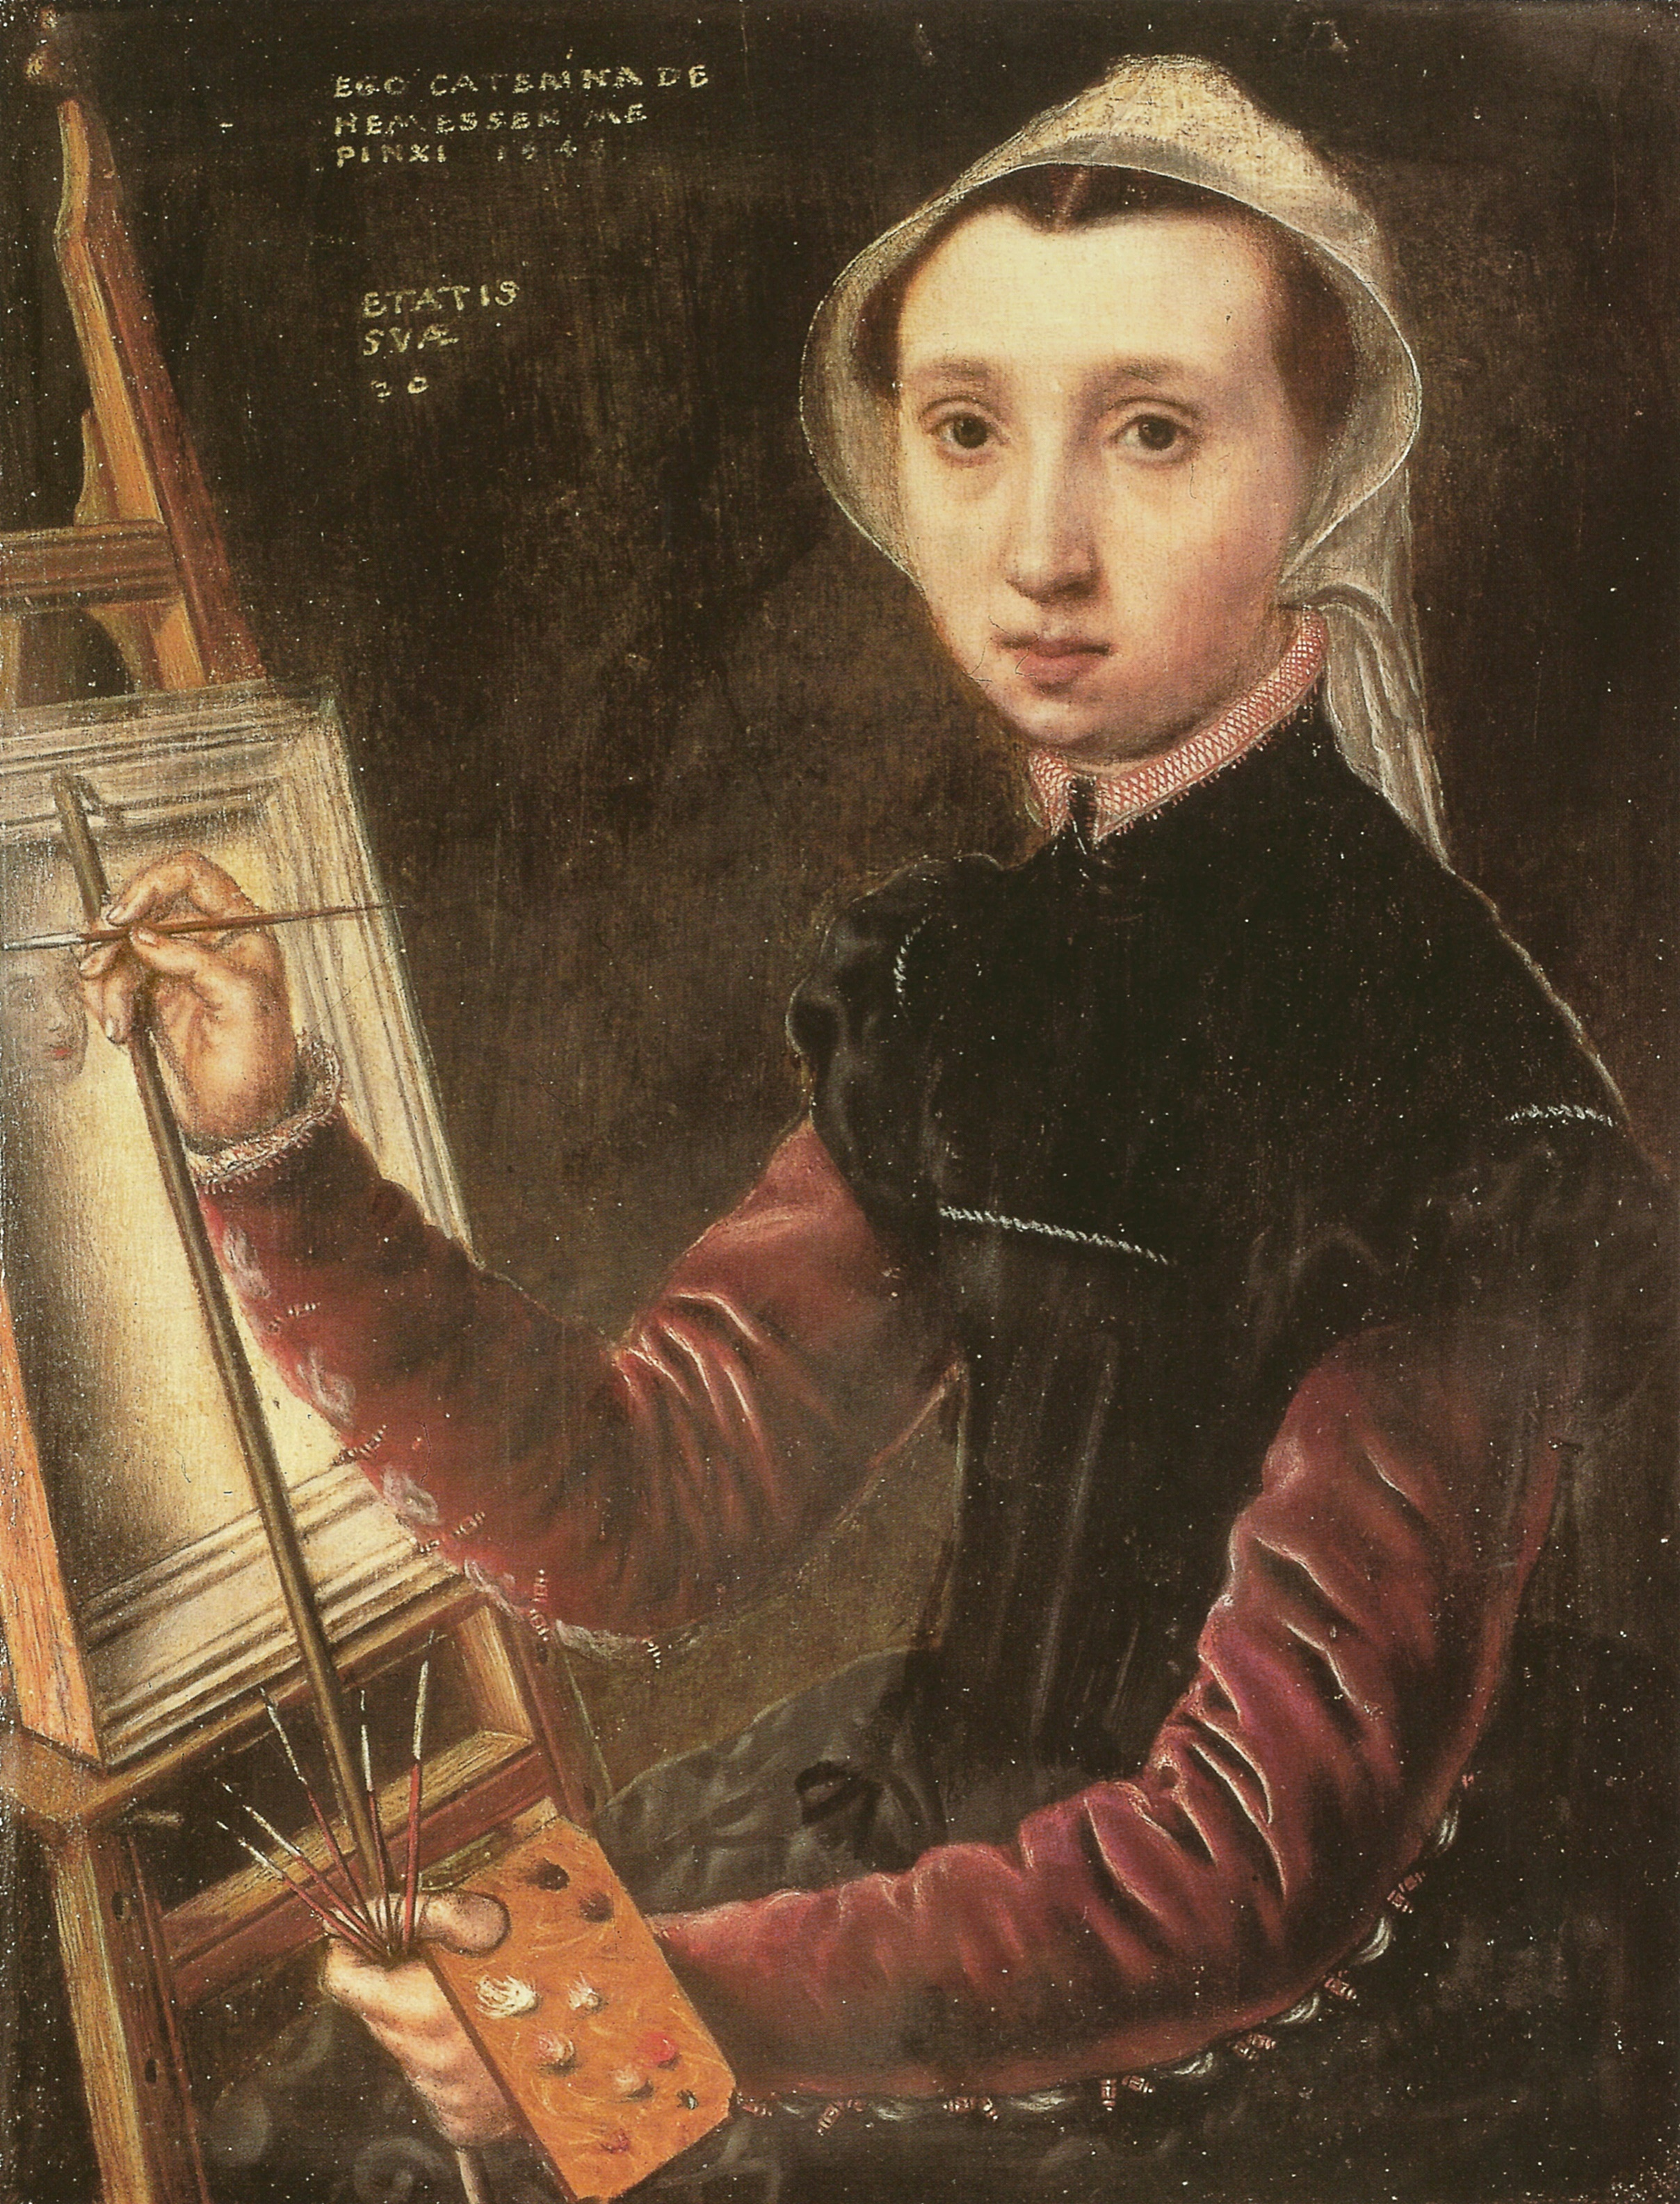
\includegraphics[width=0.3\linewidth]{self-portrait}
	\caption{\textit{Autorretrato}}
	\label{fig:wrapfig}
\end{figure}

\begin{figure}[h]
	\centering
	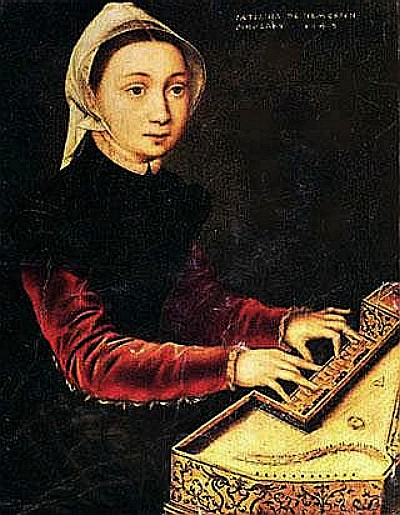
\includegraphics[width=0.4\linewidth]{portrait-of-a-22-year-old-woman-playing-the-spinet}
	\caption{\textit{Retrato de una mujer de 22 años tocando la espineta}}
\end{figure}

\begin{figure}[h]
	\centering
	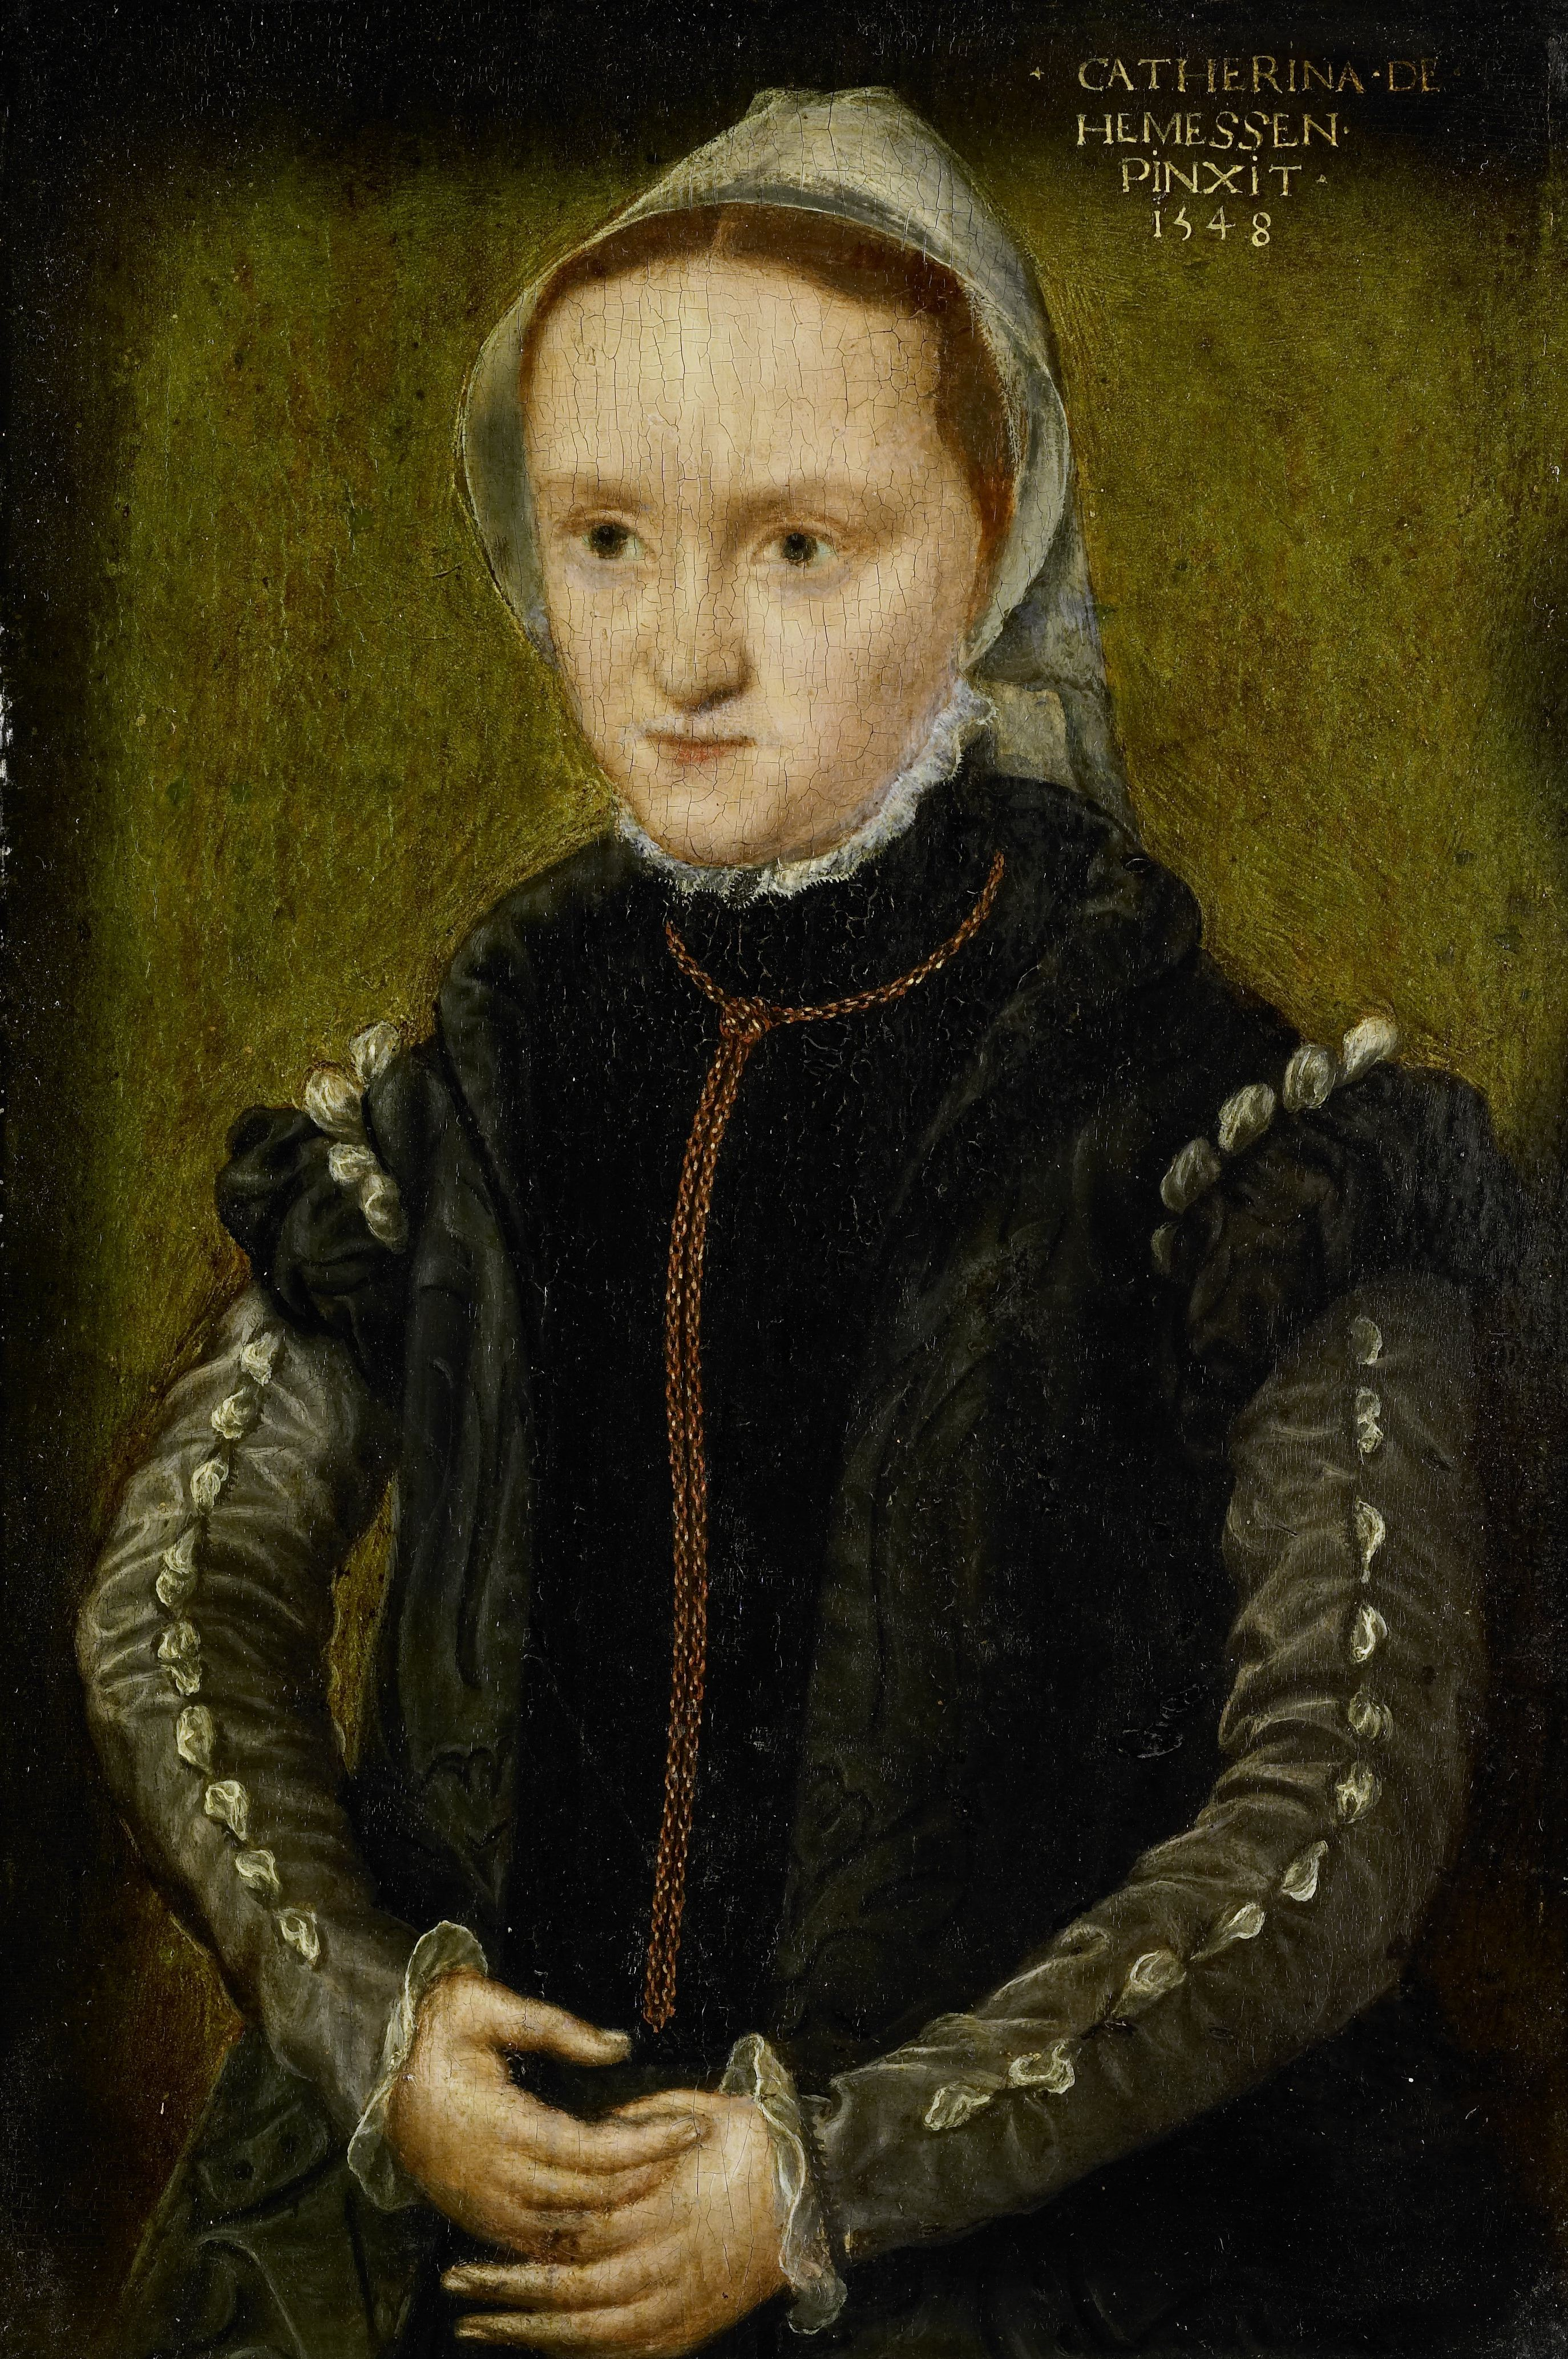
\includegraphics[width=0.4\linewidth]{portrait-of-a-woman-probably-a-self-portrait}
	\caption{\textit{Retrato de una mujer, probablemente un autorretrato}}
\end{figure}

\begin{figure}[h]
	\centering
	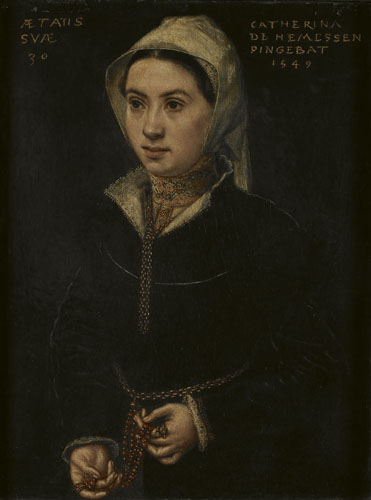
\includegraphics[width=0.4\linewidth]{portrait-of-a-30-year-old-woman}
	\caption{\textit{Retrato de una mujer de 30 años}}
\end{figure}

\begin{figure}[h]
	\centering
	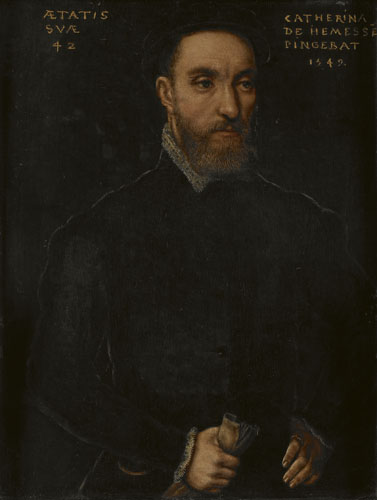
\includegraphics[width=0.4\linewidth]{portrait-of-a-42-year-old-man}
	\caption{\textit{Retrato de un hombre de 42 años}}
\end{figure}

\begin{figure}[h]
	\centering
	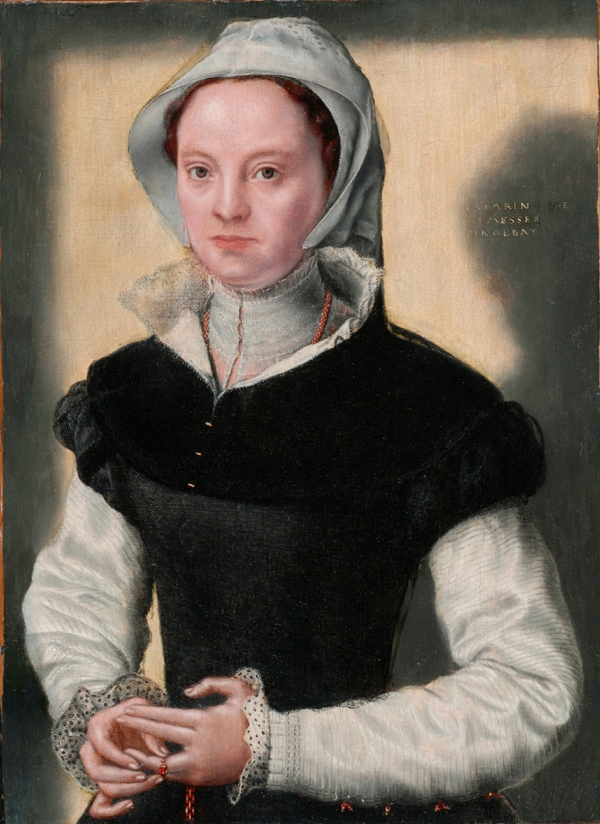
\includegraphics[width=0.4\linewidth]{portrait-of-a-young-lady}
	\caption{\textit{Retrato de una joven dama}}
\end{figure}

\begin{figure}[h]
	\centering
	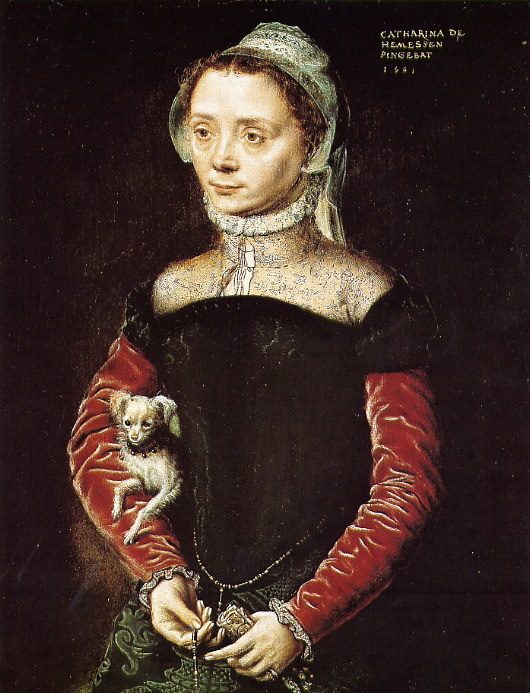
\includegraphics[width=0.4\linewidth]{portrait-of-a-woman-with-a-dog}
	\caption{\textit{Retrato de una mujer con un perro}}
\end{figure}

\begin{figure}[h]
	\centering
	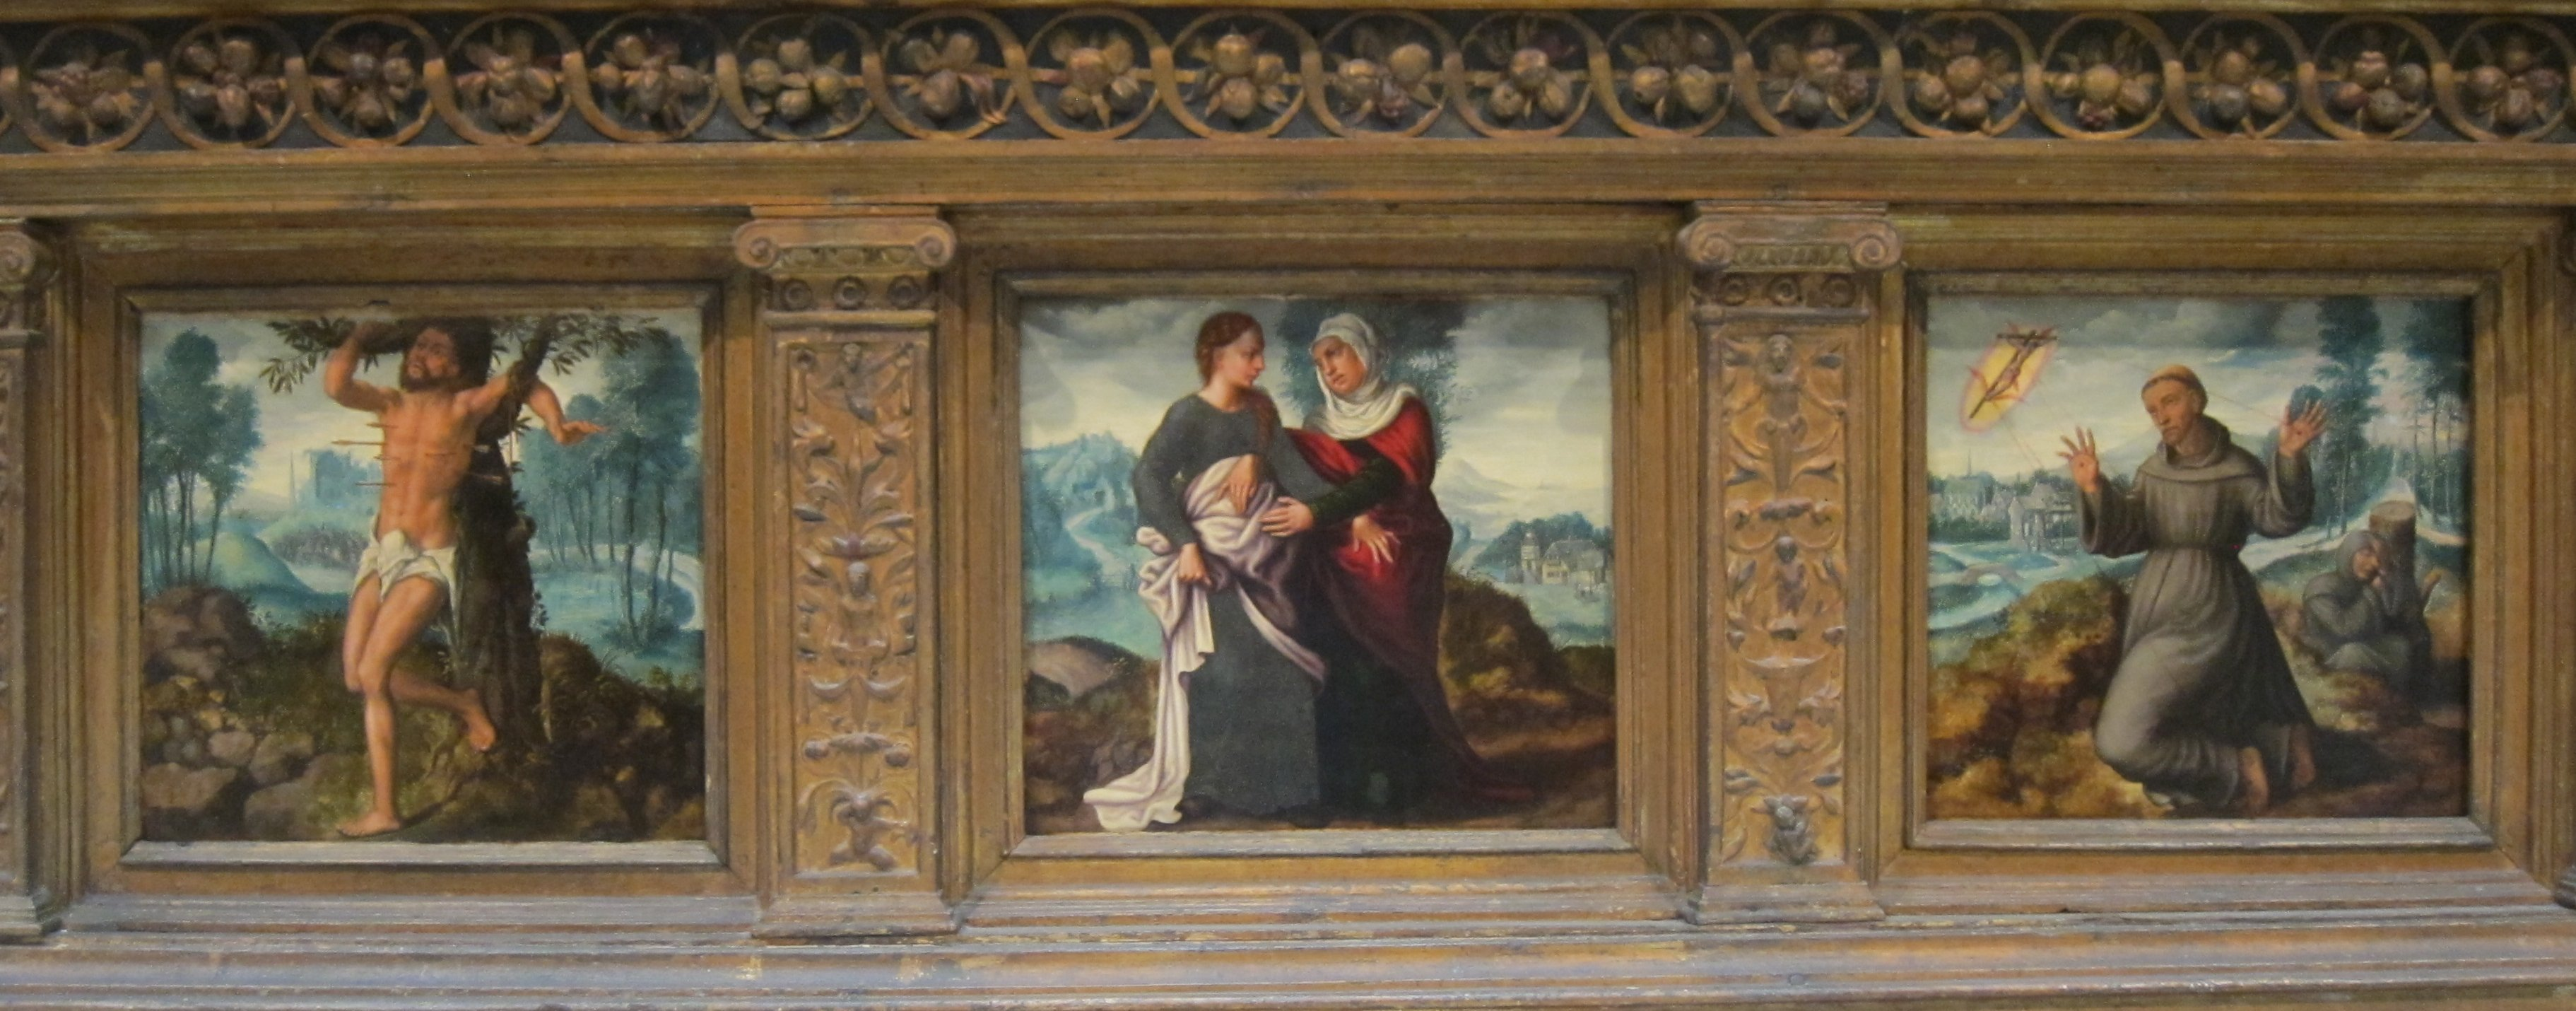
\includegraphics[width=0.8\linewidth]{predella-tendilla-retablo}
	\caption{Predela del retablo de Tendilla}
\end{figure}

\begin{figure}[h]
	\centering
	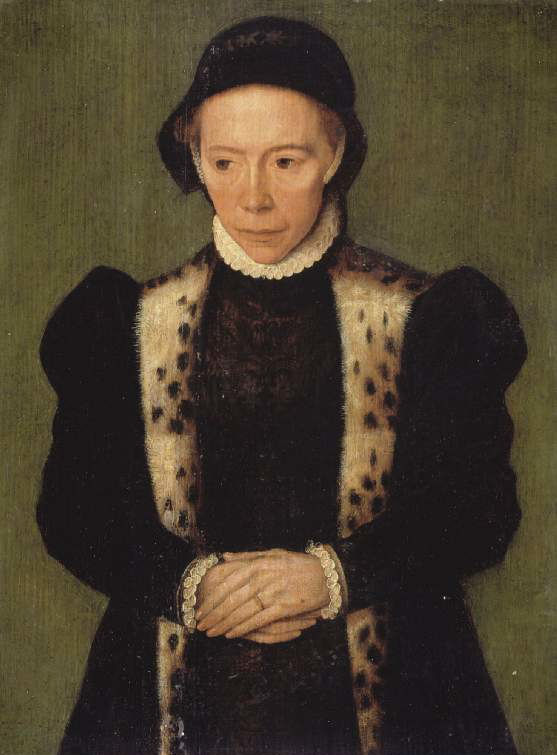
\includegraphics[width=0.4\linewidth]{portrait-of-a-woman}
	\caption{\textit{Retrato de una mujer}}
\end{figure}

\begin{figure}[h]
	\centering
	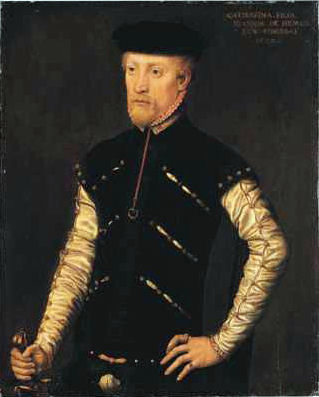
\includegraphics[width=0.4\linewidth]{portrait-of-a-man}
	\caption{\textit{Retrato de un hombre}}
\end{figure}

\begin{figure}[h]
	\centering
	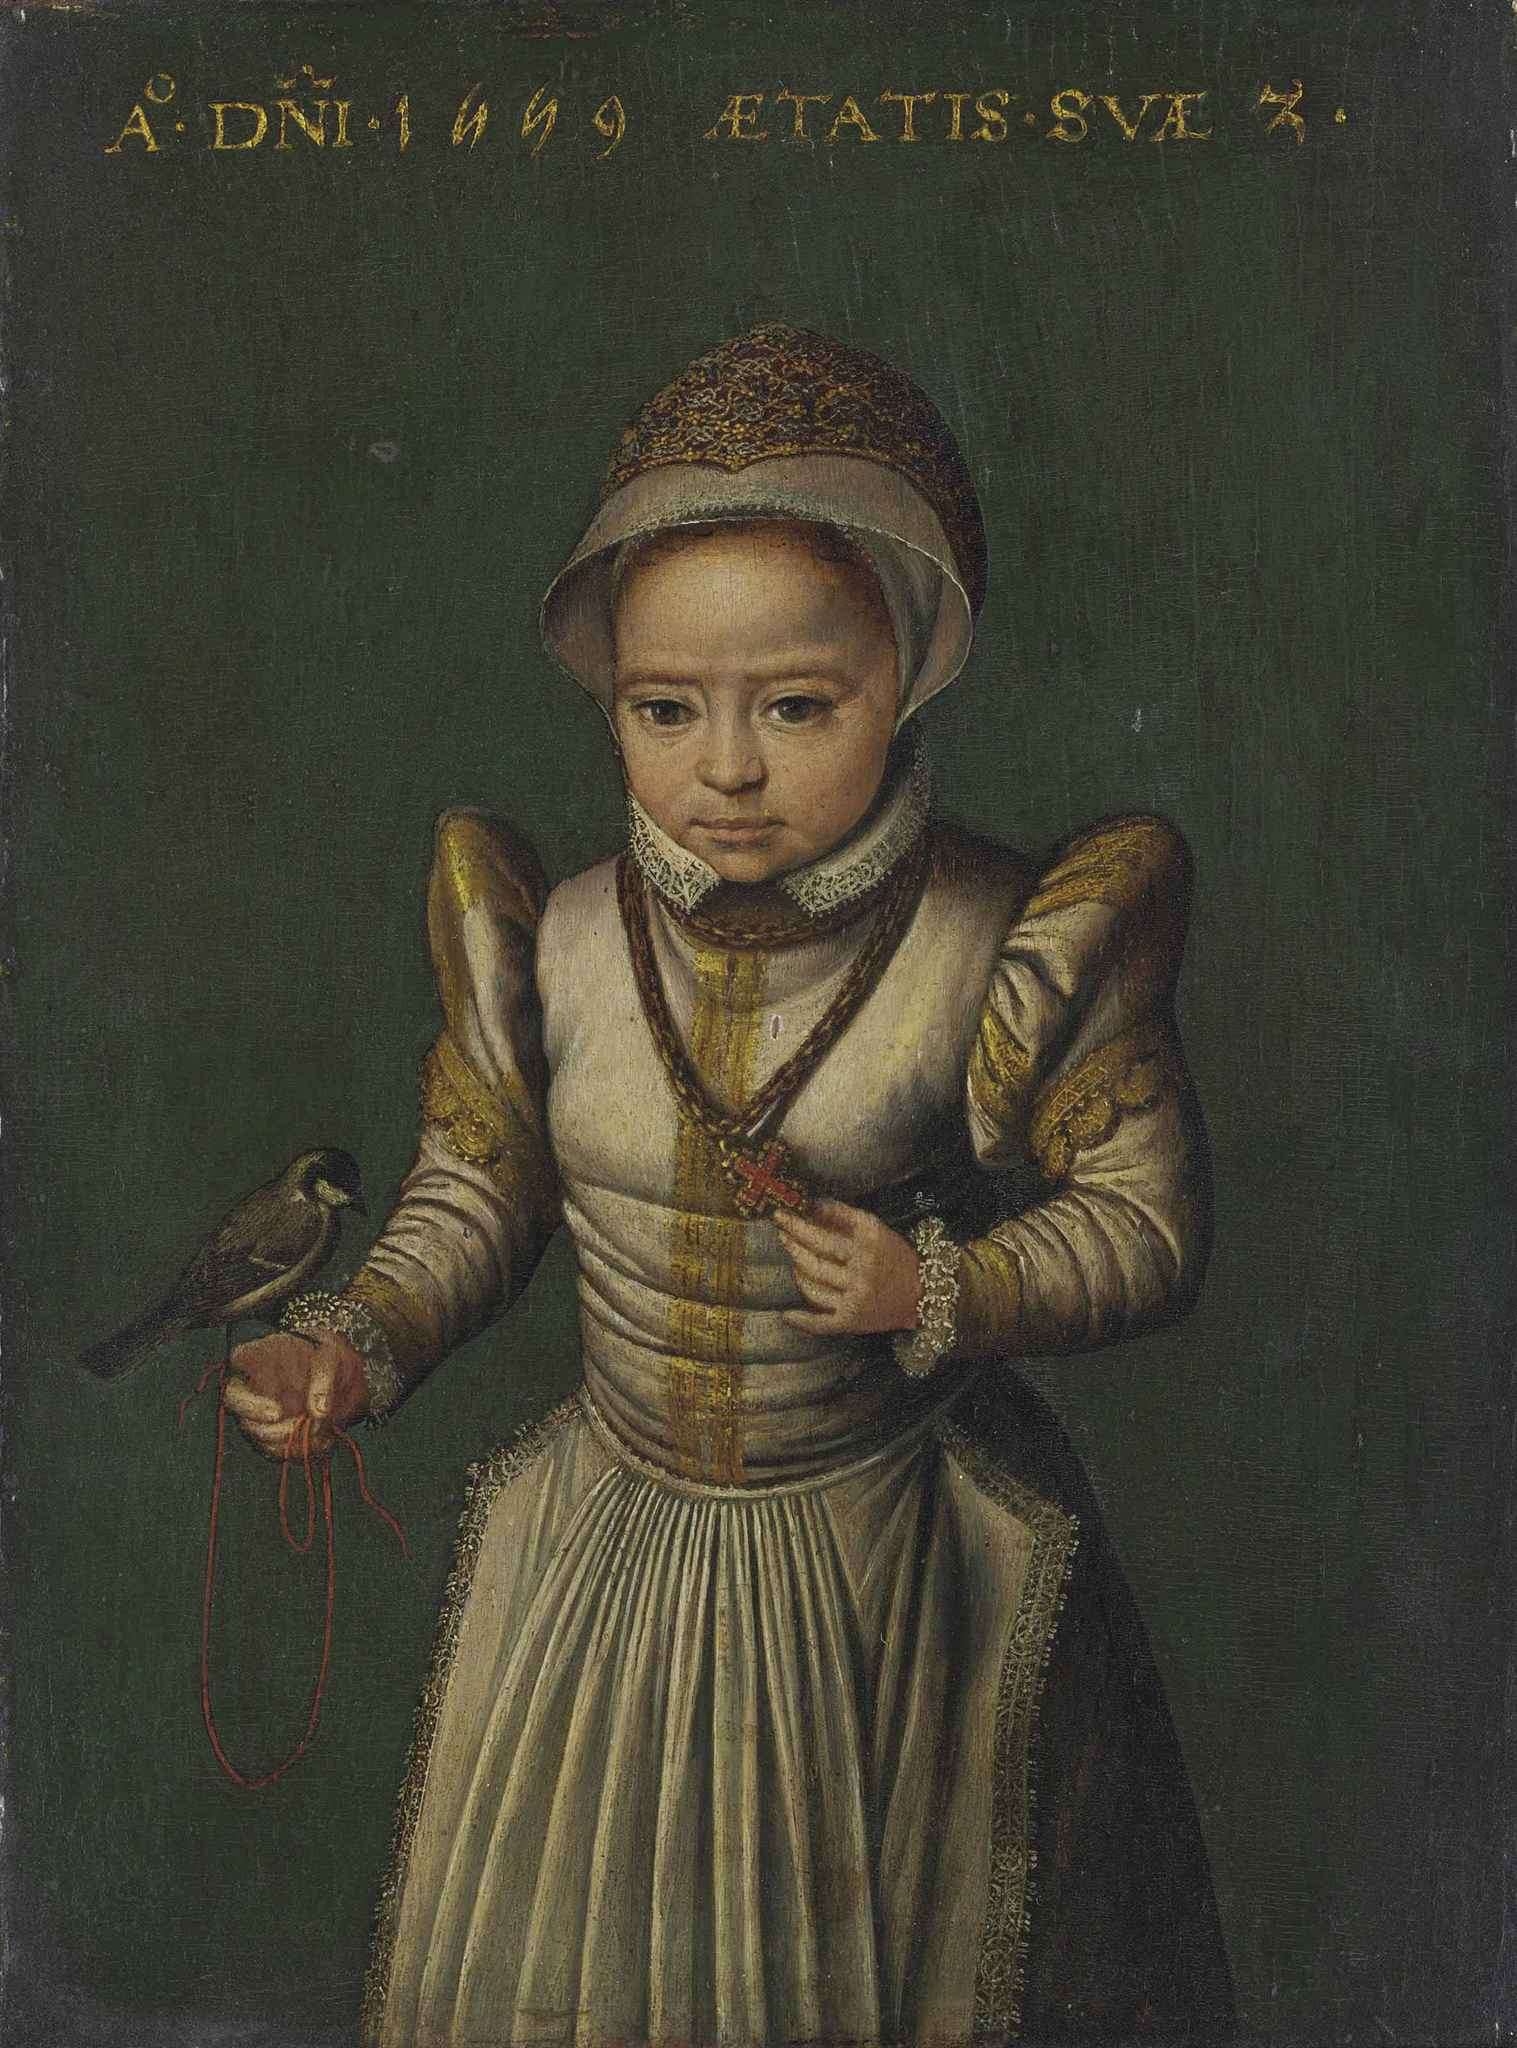
\includegraphics[width=0.4\linewidth]{portrait-of-a-child}
	\caption{\textit{Retrato de un niño}}
\end{figure}

\begin{figure}[h]
	\centering
	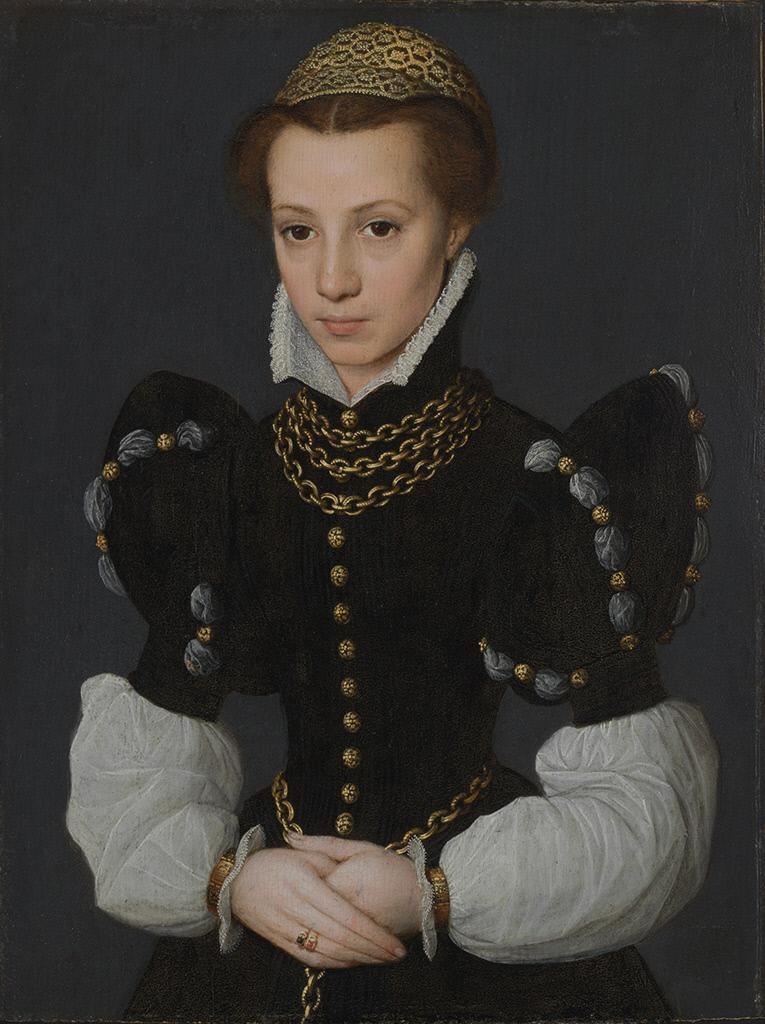
\includegraphics[width=0.4\linewidth]{portrait-of-a-young-woman}
	\caption{\textit{Retrato de una joven dama}}
\end{figure}

\begin{figure}[h]
	\centering
	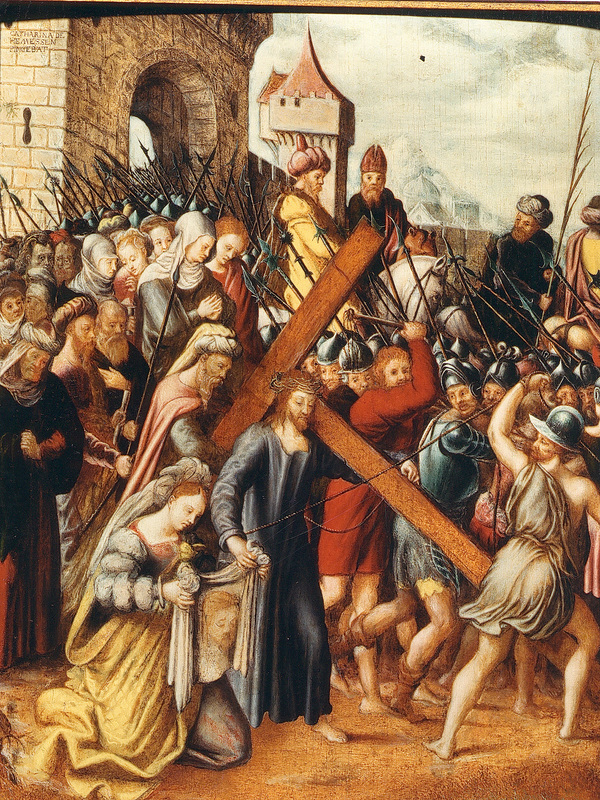
\includegraphics[width=0.4\linewidth]{christ-meets-veronica}
	\caption{\textit{Cristo se encuentra a Verónica}}
	\vspace{-20pt}
\end{figure}

\chapter{Conclusiones}

Catharina van Hemessen, al igual que muchas otras artistas (o aspirantes a artistas) de su época, lo tuvieron muy complicado para llegar a cumplir su sueño. Catharina tuvo la suerte de contar con un padre que le ayudó a conseguirlo, y fue por ello que consiguió destacar y tener un éxito y una popularidad notables.\bigskip

No obstante, otras no tuvieron la misma suerte, y tuvieron que dedicarse a lo que tradicionalmente se designaba como ``trabajo de mujeres'': criar a los hijos, ser ama de casa... Catharina también tuvo que pasar por esto al casarse, aunque la suerte la alcanzó de nuevo y pudo, aunque ni mucho menos de la misma forma que antes, continuar de forma muy pausada y lenta con su carrera artística.\bigskip

Esto nos demuestra la crueldad con la que se consideraban las mujeres: como seres inferiores e incapaces de hacer lo que los hombres hacen. También hemos de tener en cuenta que, a pesar de todo esto, nos encontramos en el Renacimiento, donde surgen corrientes humanistas, y la figura de la mujer se ensalza un poco más, si lo comparamos con el trato y la consideración que se le daba en tiempos anteriores, como en la Edad Media. Entonces, a las mujeres se las trataba de forma pésima y estaban prácticamente vetadas de participar sobre todo en las actividades intelectuales.\bigskip

Es por ello que podemos determinar cuán inferiorizadas han estado las mujeres en tiempos pasados, si aun la visión de la mujer en el Renacimiento implicó una mejoría. Pero, desgraciadamente, aún queda camino por recorrer.

\chapter{Referencias}

\textsc{Egbert}, Kim Y. y \textsc{Peacock}, Dr. Martha L. (2013). ``Situating Caterina van Hemessen in The Canon Of Sixteenth Century Dutch Portraitists''. Brigham Young University, Provo, UT, EEUU.\\
http://jur.byu.edu/?p=5517\bigskip

\textsc{Andrula} (2007). ``Caterina van Hemessen (1528-1587)''. Mujeres Pintoras.\\
http://mujerespintoras.blogspot.com/2007/11/caterina-van-hemessen-1528-1587.html\bigskip

\textsc{Ferrer Valero}, Sandra (2012). ``El arte flamenco en femenino, Caterina van Hemessen (1528-1587)''. Mujeres en la historia.\\
https://www.mujeresenlahistoria.com/2012/06/el-arte-flamenco-en-femenino-caterina.html\bigskip

\textsc{Piccardo}, Andrea (2016). ``Caterina van Hemessen (1528-1587)''. ABC Color: Cultural.\\
https://www.abc.com.py/edicion-impresa/suplementos/cultural/caterina-van-hemessen-1528-1587-1486515.html\bigskip

\textsc{Varios Autores} (2016). ``Caterina van Hemessen''. Mujeres en el Renacimiento.\\
http://sansemujeresenelrenacimiento.blogspot.com/p/caterina-van-hemessen.html\bigskip

\textsc{Varios Autores} (2015-2020). ``Catharina van Hemessen''. EcuRed, Enciclopedia Cubana.\\
https://www.ecured.cu/Caterina_van_Hemessen\bigskip

\textsc{Varios Autores} (2008-2020). ``Catharina van Hemessen''. Wikipedia, The Free Encyclopedia.\\
https://en.wikipedia.org/wiki/Catharina_van_Hemessen\bigskip

\textsc{Varios Autores} (2015-2020). ``List of paintings by Catharina van Hemessen''. Wikipedia, The Free Encyclopedia.\\
https://en.wikipedia.org/wiki/List_of_paintings_by_Catharina_van_Hemessen\bigskip

``Self-Portrait'' (s.f.). Gosudartennyj Èrmitaž, San Petersburgo, Rusia.\\
https://www.hermitagemuseum.org/wps/portal/hermitage/digital-collection/01.\%20Paintings/38355/!ut/p/z1/jZBNT8MwDIb_Cjv0SOx-pC27RUFijI1OEx8hF5RNXRvUJlUbVolfT0BcQFDmm6XHrx8bJAiQRh11pZy2RjW-f5Lpc8FYGsYclwWnl8iK7YZu-e0Vhgk8fgL4RzEEecr8BCCn45f_LfAXRP2aryuQnXL1uTYHCwJDcrZR2jhtqgFEnMeUehf5I-36JvNpd3RRFA884skXMO2jdy0Z9y1BQiOKYXyBmGdRluTphwwzuzj3Mn15KPuyJ6-9_3Lt\bigskip

``Young woman playing a virginal'' (s.f.). Interactive Fine Art Gallery \& Museum: USEUM.\\
https://useum.org/artwork/Young-woman-playing-a-virginal-Catharina-van-Hemessen\bigskip

\textsc{Varios Autores} (2015-2019). ``Young woman playing a virginal'' (Q19186181). Wikidata.\\
https://www.wikidata.org/wiki/Q19186181\bigskip

``Young girl playing the virginal by Catharina van Hemessen (1528-1587, Belgium)'' (s.f.). WahooArt.\\
https://en.wahooart.com/@@/A2A2F4-Catharina-Van-Hemessen-Young-girl-playing-the-virginal\bigskip

\textsc{Google}, Inc. (s.f.). ``Portrait of a woman, probably a Self Portrait''. Google Arts \& Culture.\\
https://artsandculture.google.com/asset/portrait-of-a-woman-probably-a-self-portrait/ngEvO7oqnnA6gA\bigskip

``Portret van een vrouw, waarschijnlijk een zelfportret, Catharina van Hemessen, 1548'' (s.f.). Rijksmuseum, Ámsterdam, Países Bajos.\\
https://cdn.rijksmuseum.nl/en/collection/SK-A-4256\bigskip

``Portrait of a Woman, probably a Self Portrait'' (s.f.). Interactive Fine Art Gallery \& Museum: USEUM.\\
https://useum.org/artwork/Portrait-of-a-Woman-probably-a-Self-Portrait-Catharina-van-Hemessen-1548\bigskip

\textsc{Varios Autores} (2014-2020). ``Portrait of a woman (1548)'' (Q17339370). Wikidata.\\
https://www.wikidata.org/wiki/Q17339370\bigskip

``Portrait of a 30-year-old Woman'' (s.f.). Interactive Fine Art Gallery \& Museum: USEUM.\\
https://useum.org/artwork/Portrait-of-a-30-year-old-Woman-Catharina-van-Hemessen\bigskip

\textsc{Varios Autores} (2015-2019). ``Portrait of a 30-year-old Woman'' (Q19203207). Wikidata.\\
https://www.wikidata.org/wiki/Q19203207\bigskip

``Kunstwerk «Vrouwenportret»'' (s.f.). Koninklijke Musea voor Schone Kunsten van België, Bruselas, Bélgica.\\
https://www.fine-arts-museum.be/nl/de-collectie/catharina-van-hemessen-vrouwenportret\bigskip

\textsc{Anónimo} (s.f.). ``Catharina van Hemessen''. Google Sites.\\
https://sites.google.com/site/catharinavanhemessen/\bigskip

\textsc{Varios Autores} (2015-2019). ``Portrait of a Lady'' (Q19185753). Wikidata.\\
https://www.wikidata.org/wiki/Q19185753\bigskip

``Catharina van Hemessen: Portrait of a Woman'' (s.f.). National Gallery, Londres, Reino Unido.\\
https://www.nationalgallery.org.uk/paintings/catharina-van-hemessen-portrait-of-a-woman\bigskip

``Portrait of a Lady'' (s.f.). Art UK.\\
https://artuk.org/discover/artworks/portrait-of-a-lady-114862\bigskip

\textsc{Varios Autores} (2015-2019). ``Portrait of a Woman with a Dog'' (Q19191957). Wikidata.\\
https://www.wikidata.org/wiki/Q19191957\bigskip

``Altarpiece with Scenes from the Old and New Testaments (the Tendila Retablo)'' (s.f.). Cincinnati Art Museum, Cincinnati, OH, EEUU.\\
https://www.cincinnatiartmuseum.org/art/explore-the-collection?id=11315623\bigskip

\textsc{Varios Autores} (2015-2019). ``Portrait of a woman (1555)'' (Q19204095). Wikidata.\\
https://www.wikidata.org/wiki/Q19204095\bigskip

``Portrait of a woman (1555)'' (s.f.). Crotos.\\
http://zone47.com/crotos/?q=19204095\bigskip

``Catharina van Hemessen: Portrait of a Man'' (s.f.). National Gallery, Londres, Reino Unido.\\
https://www.nationalgallery.org.uk/paintings/catharina-van-hemessen-portrait-of-a-man\bigskip

``Portrait of a Man'' (s.f.). Art UK.\\
https://artuk.org/discover/artworks/portrait-of-a-man-114890\bigskip

\textsc{Obelisk} Art History, LLC. (s.f.). ``Portrait of a Man by Catharina van Hemessen''. Obelisk Art History.\\
https://arthistoryproject.com/artists/catharina-van-hemessen/portrait-of-a-man/\bigskip

``Portrait of a Child'' (s.f.). Interactive Fine Art Gallery \& Museum: USEUM.\\
https://useum.org/artwork/Portrait-of-a-Child-Catharina-van-Hemessen\bigskip

``Christ Carrying the Cross, with the Meeting with Saint Veronica'' (s.f.). Interactive Fine Art Gallery \& Museum: USEUM.\\
https://useum.org/artwork/Christ-Carrying-the-Cross-with-the-Meeting-with-Saint-Veronica-Catharina-van-Hemessen\bigskip

\textsc{Varios Autores} (2015-2019). ``Christ Carrying the Cross, with the Meeting with Saint Veronica'' (Q21055034). Wikidata.\\
https://www.wikidata.org/wiki/Q21055034\bigskip

``Christ Carrying the Cross, with the Meeting with Saint Veronica'' (s.f.). Crotos.\\
http://zone47.com/crotos/?q=21055034

\chapter{Notas}

\section{Autoría}

Este trabajo ha sido realizado por Alberto Navalón Lillo (3ESO A), acabado a día 8 de abril de 2020.

\section{Veracidad de fuentes e histórica}

Se ha intentado comprobar la veracidad de las fuentes de este documento de la forma más rigurosa posible. No obstante, se advierte de que es posible que encuentre inexactitudes históricas entre el contenido.

\section{Derechos de autor}

Este trabajo se encuentra bajo la licencia Creative Commons Atribución/Reconocimiento-NoComercial 4.0 Internacional (CC BY-NC). Para obtener más información acerca de esta licencia y los permisos que se obtienen al aplicarse, refiérase a:\\
https://creativecommons.org/licenses/by-nc/4.0/legalcode.es
\begin{figure}[h]
	\centering
	
\includegraphics[height=1cm]{cc-by-nc}
\end{figure}

\end{document}

%%%% REFERENCES %%%%
% https://en.wikipedia.org/wiki/Catharina_van_Hemessen
% http://jur.byu.edu/?p=5517
% https://www.ecured.cu/Caterina_van_Hemessen
% http://mujerespintoras.blogspot.com/2007/11/caterina-van-hemessen-1528-1587.html
% https://www.mujeresenlahistoria.com/2012/06/el-arte-flamenco-en-femenino-caterina.html
% https://www.abc.com.py/edicion-impresa/suplementos/cultural/caterina-van-hemessen-1528-1587-1486515.html
% http://sansemujeresenelrenacimiento.blogspot.com/p/caterina-van-hemessen.html
% https://en.wikipedia.org/wiki/List_of_paintings_by_Catharina_van_Hemessen

% 1. SELF-PORTRAIT
%% https://www.hermitagemuseum.org/wps/portal/hermitage/digital-collection/01.%20Paintings/38355/!ut/p/z1/jZBNT8MwDIb_Cjv0SOx-pC27RUFijI1OEx8hF5RNXRvUJlUbVolfT0BcQFDmm6XHrx8bJAiQRh11pZy2RjW-f5Lpc8FYGsYclwWnl8iK7YZu-e0Vhgk8fgL4RzEEecr8BCCn45f_LfAXRP2aryuQnXL1uTYHCwJDcrZR2jhtqgFEnMeUehf5I-36JvNpd3RRFA884skXMO2jdy0Z9y1BQiOKYXyBmGdRluTphwwzuzj3Mn15KPuyJ6-9_3LtXDfMAwxwHEdSWVs1JdnbNsDfRmo7OBDfSejae_G2WuALbY4rNpu9A14z5fQ!/dz/d5/L2dBISEvZ0FBIS9nQSEh/?lng=en

% 2. PORTRAIT OF A 22-YEAR-OLD WOMAN PLAYING THE SPINET
%% https://useum.org/artwork/Young-woman-playing-a-virginal-Catharina-van-Hemessen
%% https://www.wikidata.org/wiki/Q19186181
%% https://en.wahooart.com/@@/A2A2F4-Catharina-Van-Hemessen-Young-girl-playing-the-virginal

% 3. PORTRAIT OF A WOMAN, PROBABLY A SELF-PORTRAIT
%% https://artsandculture.google.com/asset/portrait-of-a-woman-qprobably-a-self-portrait/ngEvO7oqnnA6gA
%% https://cdn.rijksmuseum.nl/en/collection/SK-A-4256
%% https://useum.org/artwork/Portrait-of-a-Woman-probably-a-Self-Portrait-Catharina-van-Hemessen-1548
%% https://www.wikidata.org/wiki/Q17339370

% 4. PORTRAIT OF A 30-YEAR-OLD WOMAN
%% https://useum.org/artwork/Portrait-of-a-30-year-old-Woman-Catharina-van-Hemessen
%% https://www.wikidata.org/wiki/Q19203207
%% https://www.fine-arts-museum.be/nl/de-collectie/catharina-van-hemessen-vrouwenportret
%% http://zone47.com/crotos/?q=19203207

% 5. PORTRAIT OF A 42-YEAR-OLD MAN
% https://useum.org/artwork/Portrait-of-a-42-year-old-Man-Catharina-van-Hemessen
% https://www.wikidata.org/wiki/Q19203163
% https://www.fine-arts-museum.be/nl/de-collectie/catharina-van-hemessen-mansportret
% https://sites.google.com/site/catharinavanhemessen/

% 6. PORTRAIT OF A YOUNG LADY
%% https://www.wikidata.org/wiki/Q19185753

% 7. PORTRAIT OF A WOMAN WITH A DOG
%% https://www.nationalgallery.org.uk/paintings/catharina-van-hemessen-portrait-of-a-woman
%% https://artuk.org/discover/artworks/portrait-of-a-lady-114862
%% https://www.wikidata.org/wiki/Q19191957

% 8. PREDELLA OF THE TENDILLA RETABLO
%% https://www.cincinnatiartmuseum.org/art/explore-the-collection?id=11315623

% 9. PORTRAIT OF A WOMAN
%% https://www.wikidata.org/wiki/Q19204095
%% http://zone47.com/crotos/?q=19204095

% 10. PORTRAIT OF A MAN
%% https://www.nationalgallery.org.uk/paintings/catharina-van-hemessen-portrait-of-a-man
%% https://artuk.org/discover/artworks/portrait-of-a-man-114890
%% https://arthistoryproject.com/artists/catharina-van-hemessen/portrait-of-a-man/

% 11. PORTRAIT OF A CHILD
%% https://arthistoryproject.com/artists/catharina-van-hemessen/portrait-of-a-child/
%% https://useum.org/artwork/Portrait-of-a-Child-Catharina-van-Hemessen

% 12. PORTRAIT OF A YOUNG WOMAN
%% [NONE]

% 13. CHRIST MEETS VERONICA
%% https://useum.org/artwork/Christ-Carrying-the-Cross-with-the-Meeting-with-Saint-Veronica-Catharina-van-Hemessen
%% https://www.wikidata.org/wiki/Q21055034
%% http://zone47.com/crotos/?q=21055034